\chapter{System Analysis}

\section{Introduction}
This chapter presents a comprehensive architectural analysis of \textbf{Questro}, the integrated movie and game recommendation system. By leveraging Unified Modeling Language (UML) standards, we dissect the system's structural components, cross-domain data flows, and complex user interactions.

The analysis focuses on how the system bridges the gap between two distinct entertainment domains—cinema and gaming—using a unified profile architecture. Through the following diagrams, we visualize the transition from abstract requirements to concrete logic, ensuring a robust foundation for the implementation phase.

\section{System Requirements}
This section delineates the functional and non-functional requirements that govern the system's capabilities and performance standards.

\subsection{Functional Requirements}
These requirements define the specific behaviors and functions the system provides to end-users and administrators.

\begin{itemize}
    \item \textbf{User \& Identity Management}
    \begin{itemize}
        \item \textbf{Secure Authentication:} Support for registration, login, and password management with encryption.
        \item \textbf{Profile Customization:} Users can manage avatars, personal bios, and visibility settings.
        \item \textbf{Gamification:} The system awards \textbf{Badges} to users based on engagement milestones to encourage activity.
    \end{itemize}

    \item \textbf{Discovery \& Recommendation Engine}
    \begin{itemize}
        \item \textbf{Hybrid Recommendations:} Suggestions based on a mix of user history, collaborative filtering, and content metadata.
        \item \textbf{Surprise Me Feature:} A randomized discovery engine for users seeking novel content outside their usual preferences.
        \item \textbf{Advanced Filtering:} Search capabilities filtering by genre, release date, rating, and platform.
    \end{itemize}

    \item \textbf{Social \& Community Interaction}
    \begin{itemize}
        \item \textbf{Social Graph:} Users can follow others, viewing "friendship metrics" and shared interests.
        \item \textbf{Sentiment-Aware Reviews:} Users can review content; the system analyzes the text sentiment (Positive/Negative) to refine recommendations.
        \item \textbf{Privacy Controls:} Granular visibility settings for posts (e.g., Public, Friends Only, Private).
    \end{itemize}

    \item \textbf{Parental Control \& Safety}
    \begin{itemize}
        \item \textbf{Content Filtering:} Parents can restrict access to specific genres or age ratings.
        \item \textbf{Social Restrictions:} Parents can disable or filter chat and social interactions for child accounts.
    \end{itemize}
\end{itemize}

\subsection{Non-Functional Requirements}
These requirements define the quality attributes ensuring the system's reliability and user experience.

\begin{itemize}
    \item \textbf{Performance:} Recommendation inference latency should remain under 200ms; general page loads under 2 seconds.
    \item \textbf{Scalability:} The architecture must support horizontal scaling to handle spikes in concurrent users (10,000+).
    \item \textbf{Availability:} The system aims for 99.9\% uptime with redundancy for critical database nodes.
    \item \textbf{Security:} Strict adherence to data protection standards (GDPR compliance), including hashing of credentials and sanitization of user inputs.
\end{itemize}

\section{Use Case Modeling}
\label{sec:use_case}
The Use Case diagram captures the system's functional requirements from the user's perspective, identifying the actors and their interactions with the system.

As illustrated in Figure \ref{fig:Use_case_diagram}, the primary actors are the \textbf{End User}, who interacts with the recommendation and social features, and the \textbf{System Administrator}, who manages content moderation and user reports.
\begin{figure}[H]
    \centering
    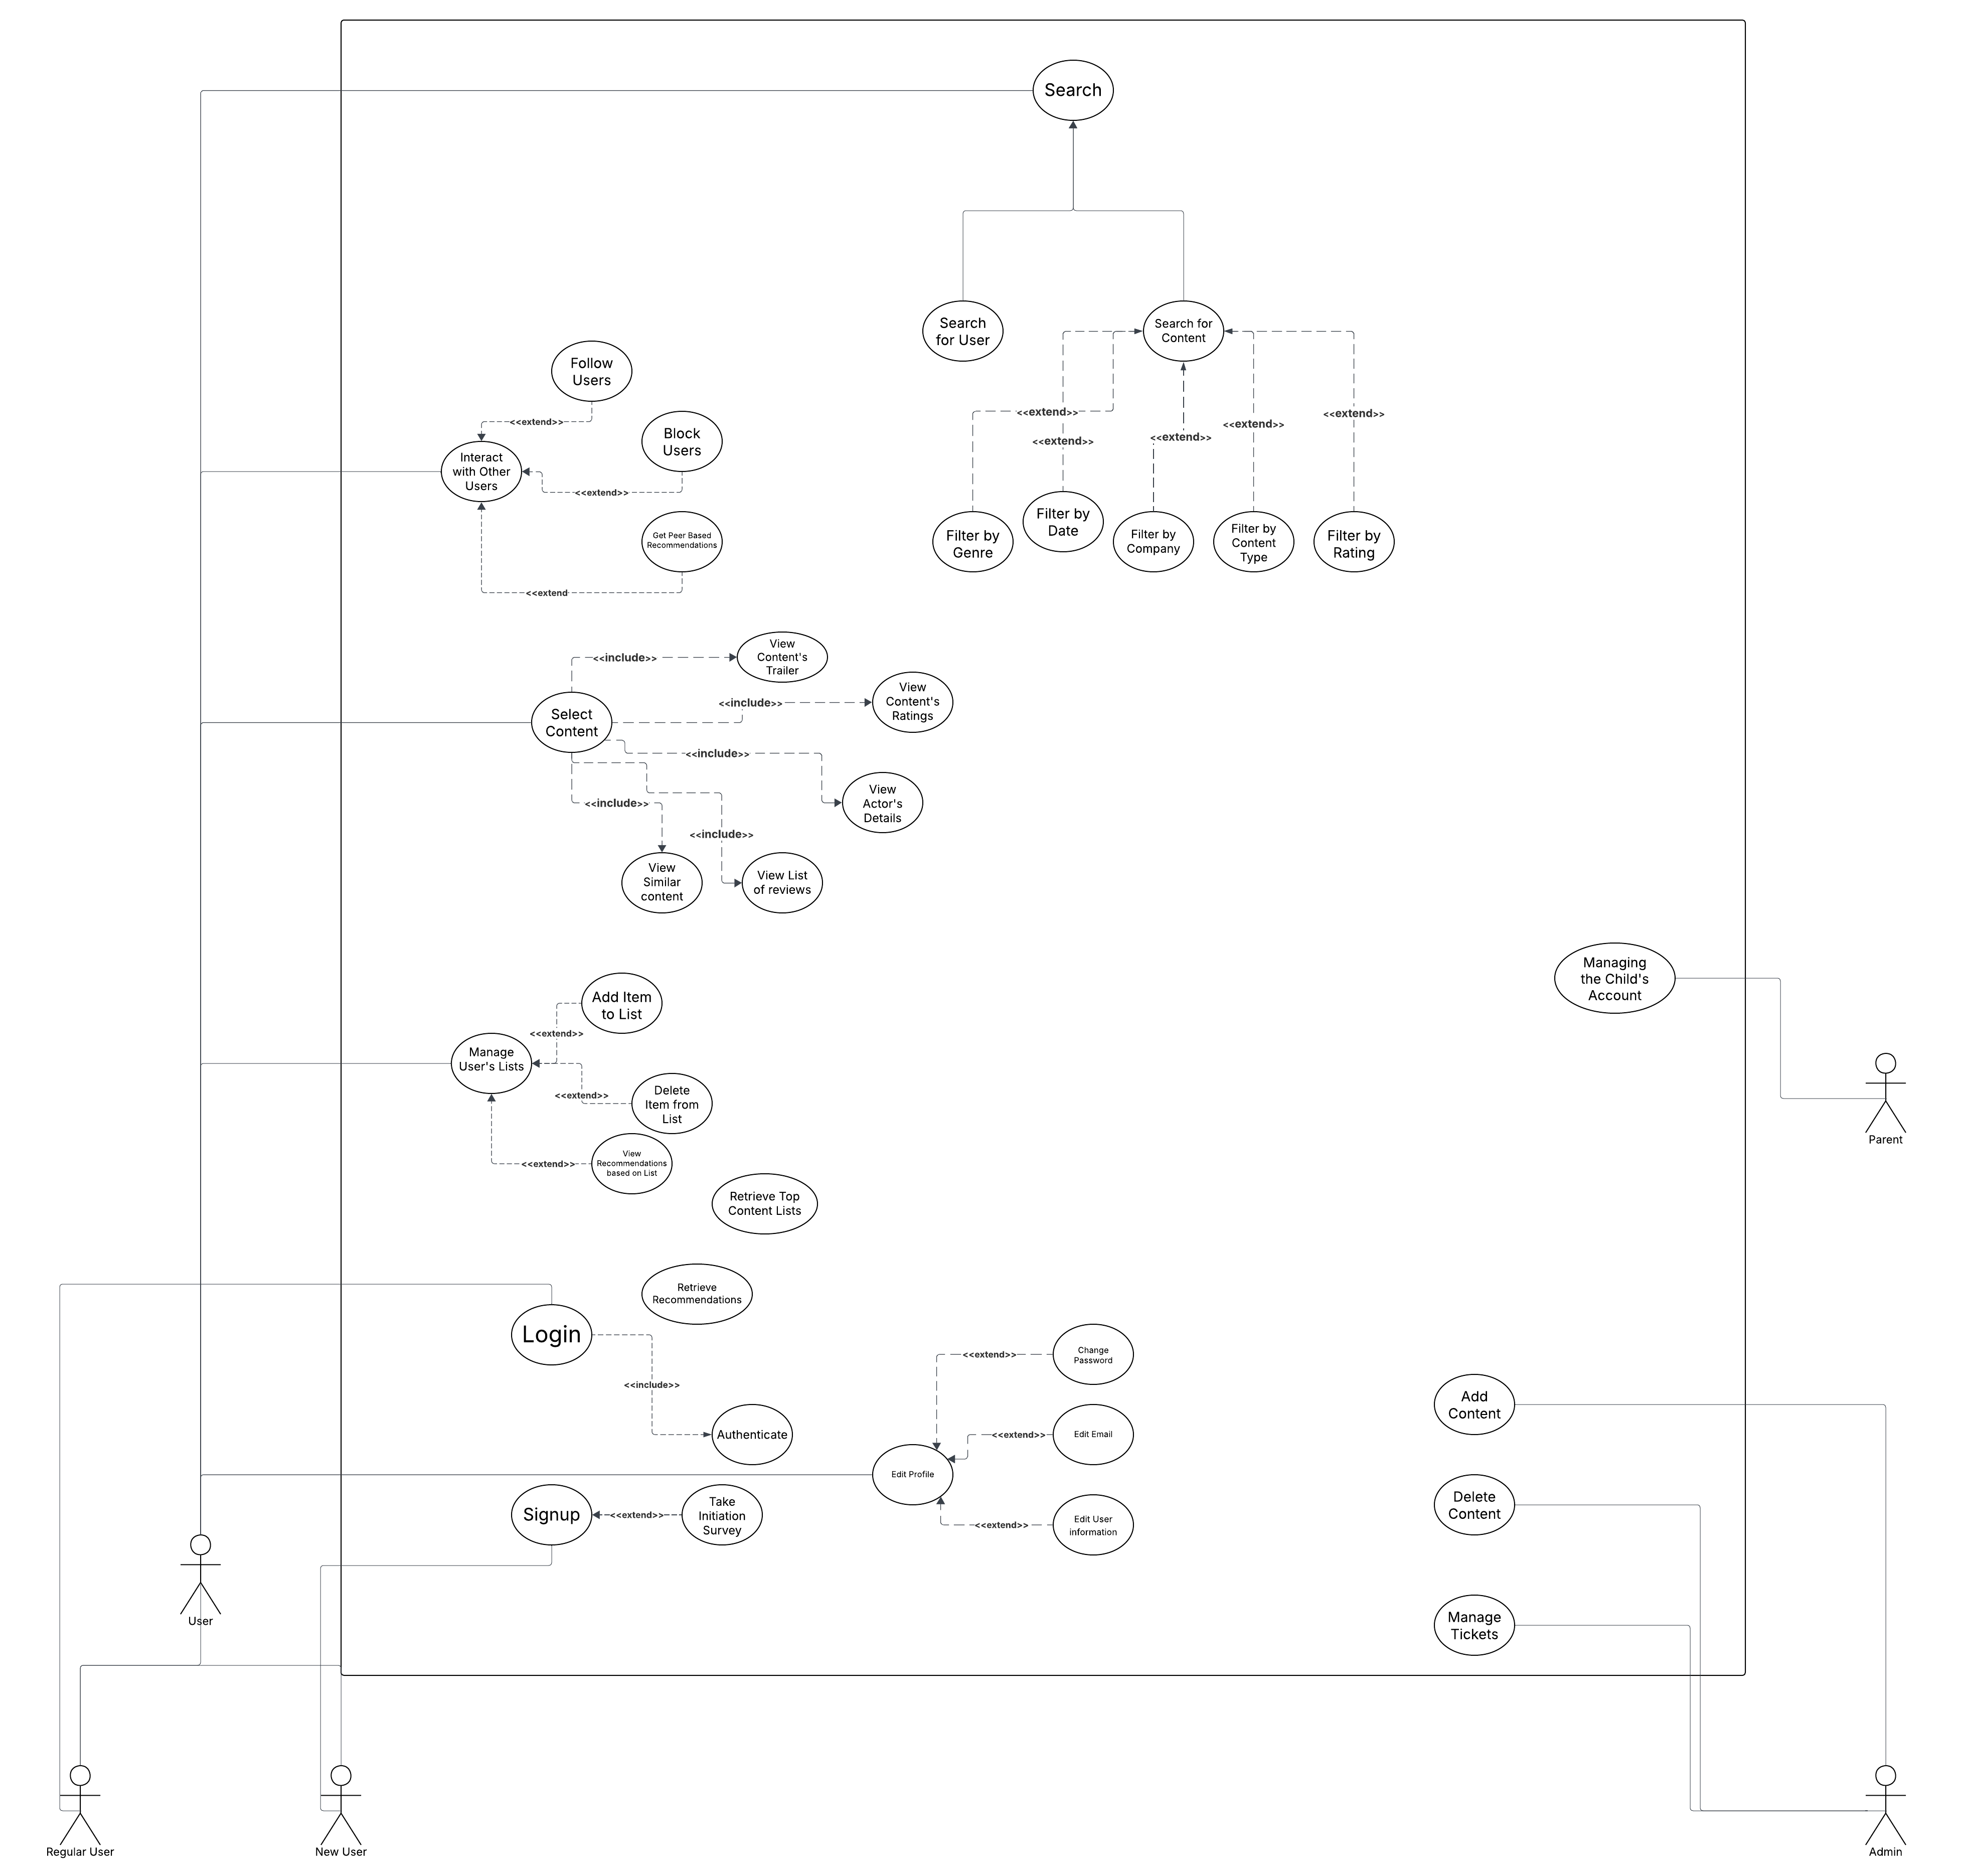
\includegraphics[width=1.0\linewidth]{figures/diagram/UseCase.png} 
    \caption{System Activity Diagram}   
    \label{fig:Use_case_diagram}
\end{figure}

\clearpage


\section{Activity Diagram}
\label{sec:activity_diagram}
The Activity Diagram (Figure \ref{fig:activity_diagram}) models the sequential flow of activities within the Questro ecosystem, illustrating the end-to-end logic from user initiation to system response. It details the operational workflows for key processes such as user authentication, content discovery, and social interaction.

The flow begins with the \textbf{Authentication Phase}, where the system verifies user credentials or directs new visitors through the onboarding process, including the "Cold Start" interest survey. Upon successful login, the control flow branches into parallel operational threads:

\begin{itemize}
    \item \textbf{Content Interaction:} This path handles the user's engagement with media, including searching, rating, and adding items to watchlists. Each interaction triggers an update to the user's profile vector in the database.
    \item \textbf{Social Engagement:} This branch manages community features, enabling users to follow peers, post reviews, and share playlists. The system checks privacy settings (e.g., Public vs. Friends Only) before committing these actions to the social graph.
    \item \textbf{Recommendation Logic:} In the background, the recommendation engine continuously processes the updated user history. It executes hybrid filtering algorithms to refresh the personalized "For You" feed, ensuring that new suggestions reflect the most recent user activities.
\end{itemize}

The diagram further illustrates exception handling, such as invalid login attempts or restricted content access (e.g., parental controls), ensuring the system degrades gracefully and provides informative feedback to the user.
\begin{figure}[H]
    \centering
    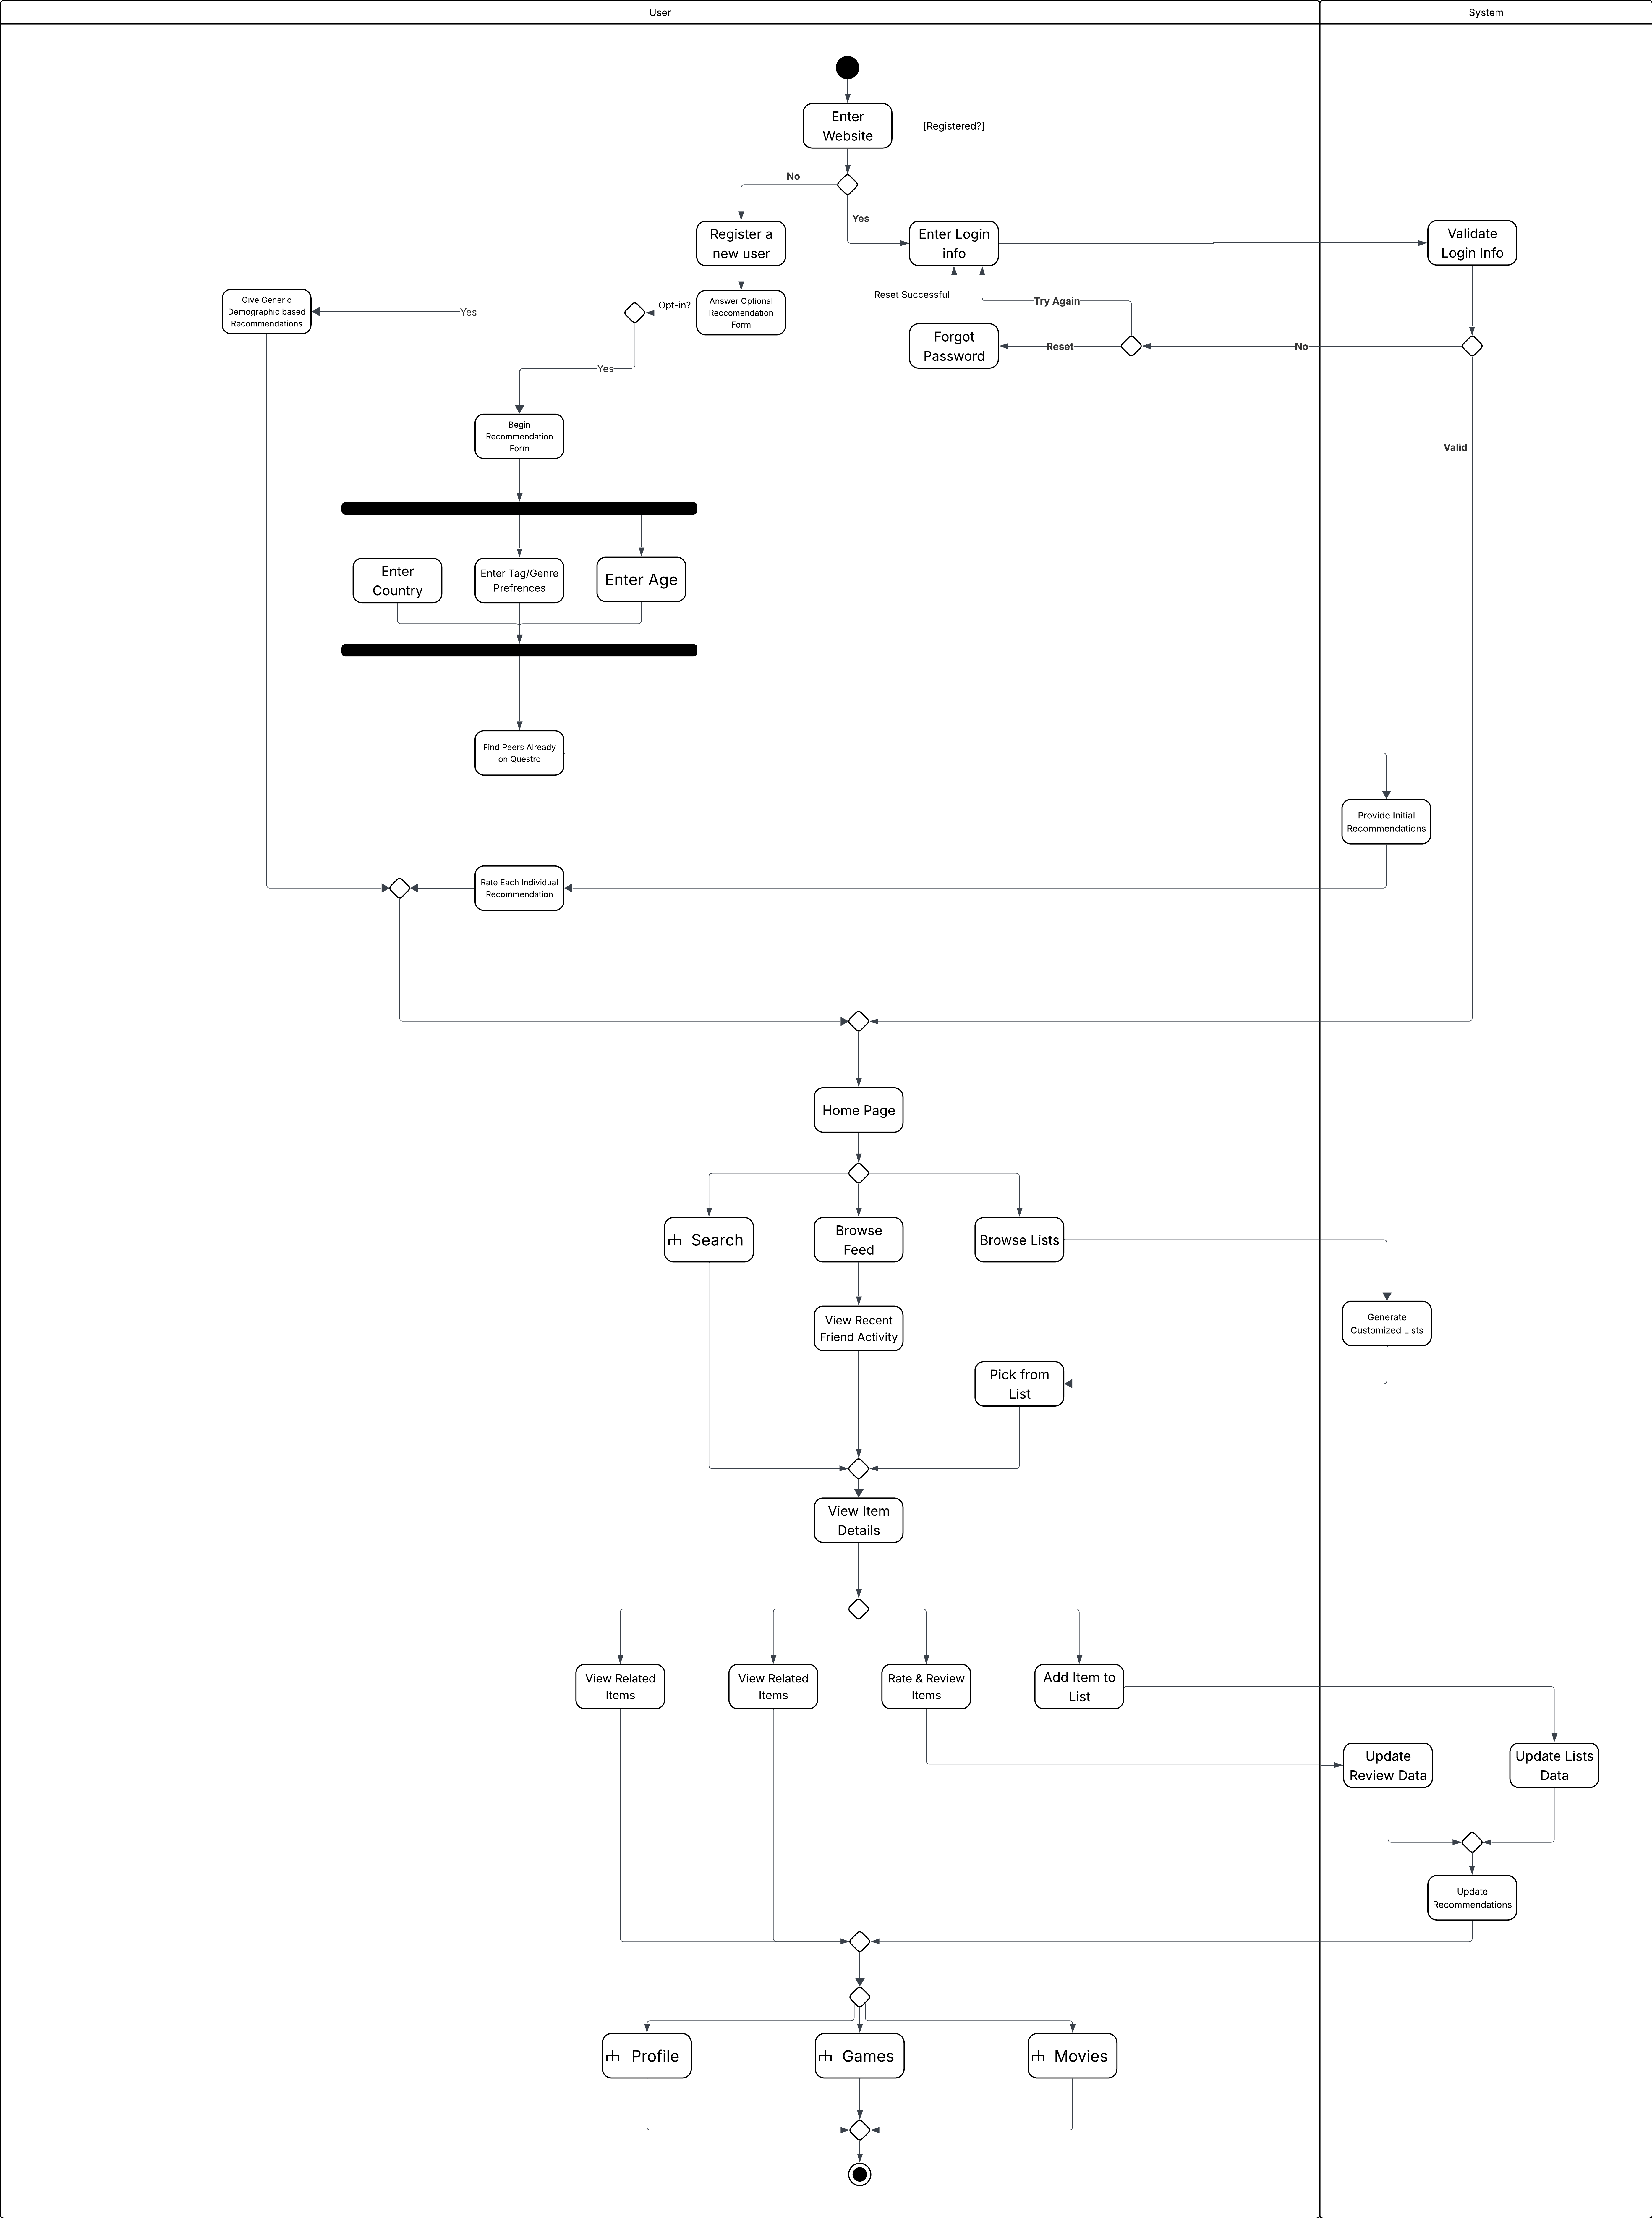
\includegraphics[width=1.0\linewidth]{figures/diagram/Activity.png}
    \caption{System Activity Diagram}
    \label{fig:activity_diagram}
\end{figure}

\section{Context Diagram}
\label{sec:context_diagram}
The Context Diagram (Figure \ref{fig:context_diagram}) establishes the operational boundaries of the Questro system, visualizing the entire platform as a single, high-level process (Process 0) interacting with its external environment. This Level 0 Data Flow Diagram identifies the primary sources of data and the recipients of system information, clarifying the scope of the project.

As depicted, the system orchestrates data exchange between three critical external entities:

\begin{itemize}
    \item \textbf{The End User:} Represents the primary actor who initiates sessions. The user provides inputs such as registration data, search queries, ratings, and reviews. In return, the system acts as an information provider, delivering personalized recommendation lists, social feeds, and profile analytics.
    
    \item \textbf{External Data Providers (TMDB \& RAWG):} Questro functions as a data aggregator that relies on third-party APIs to maintain a comprehensive catalog. It fetches cinematic metadata (cast, plot, release dates) from \textbf{TMDB} and video game attributes (platforms, developers, genres) from \textbf{RAWG}. This integration ensures the content database remains synchronized with real-world releases without manual administrative entry.

    \item \textbf{ML Inference Engine:} The architecture treats the Machine Learning model as a distinct external processing unit. The main application sends sanitized user behavior vectors and interaction logs to this engine. In response, the engine returns a list of predicted Item IDs, which the system then enriches with metadata before presenting them to the user.
\end{itemize}

This high-level abstraction ensures that all external interfaces and data dependencies are clearly defined before decomposing the system into internal subsystems.

\begin{sidewaysfigure}
    \centering
    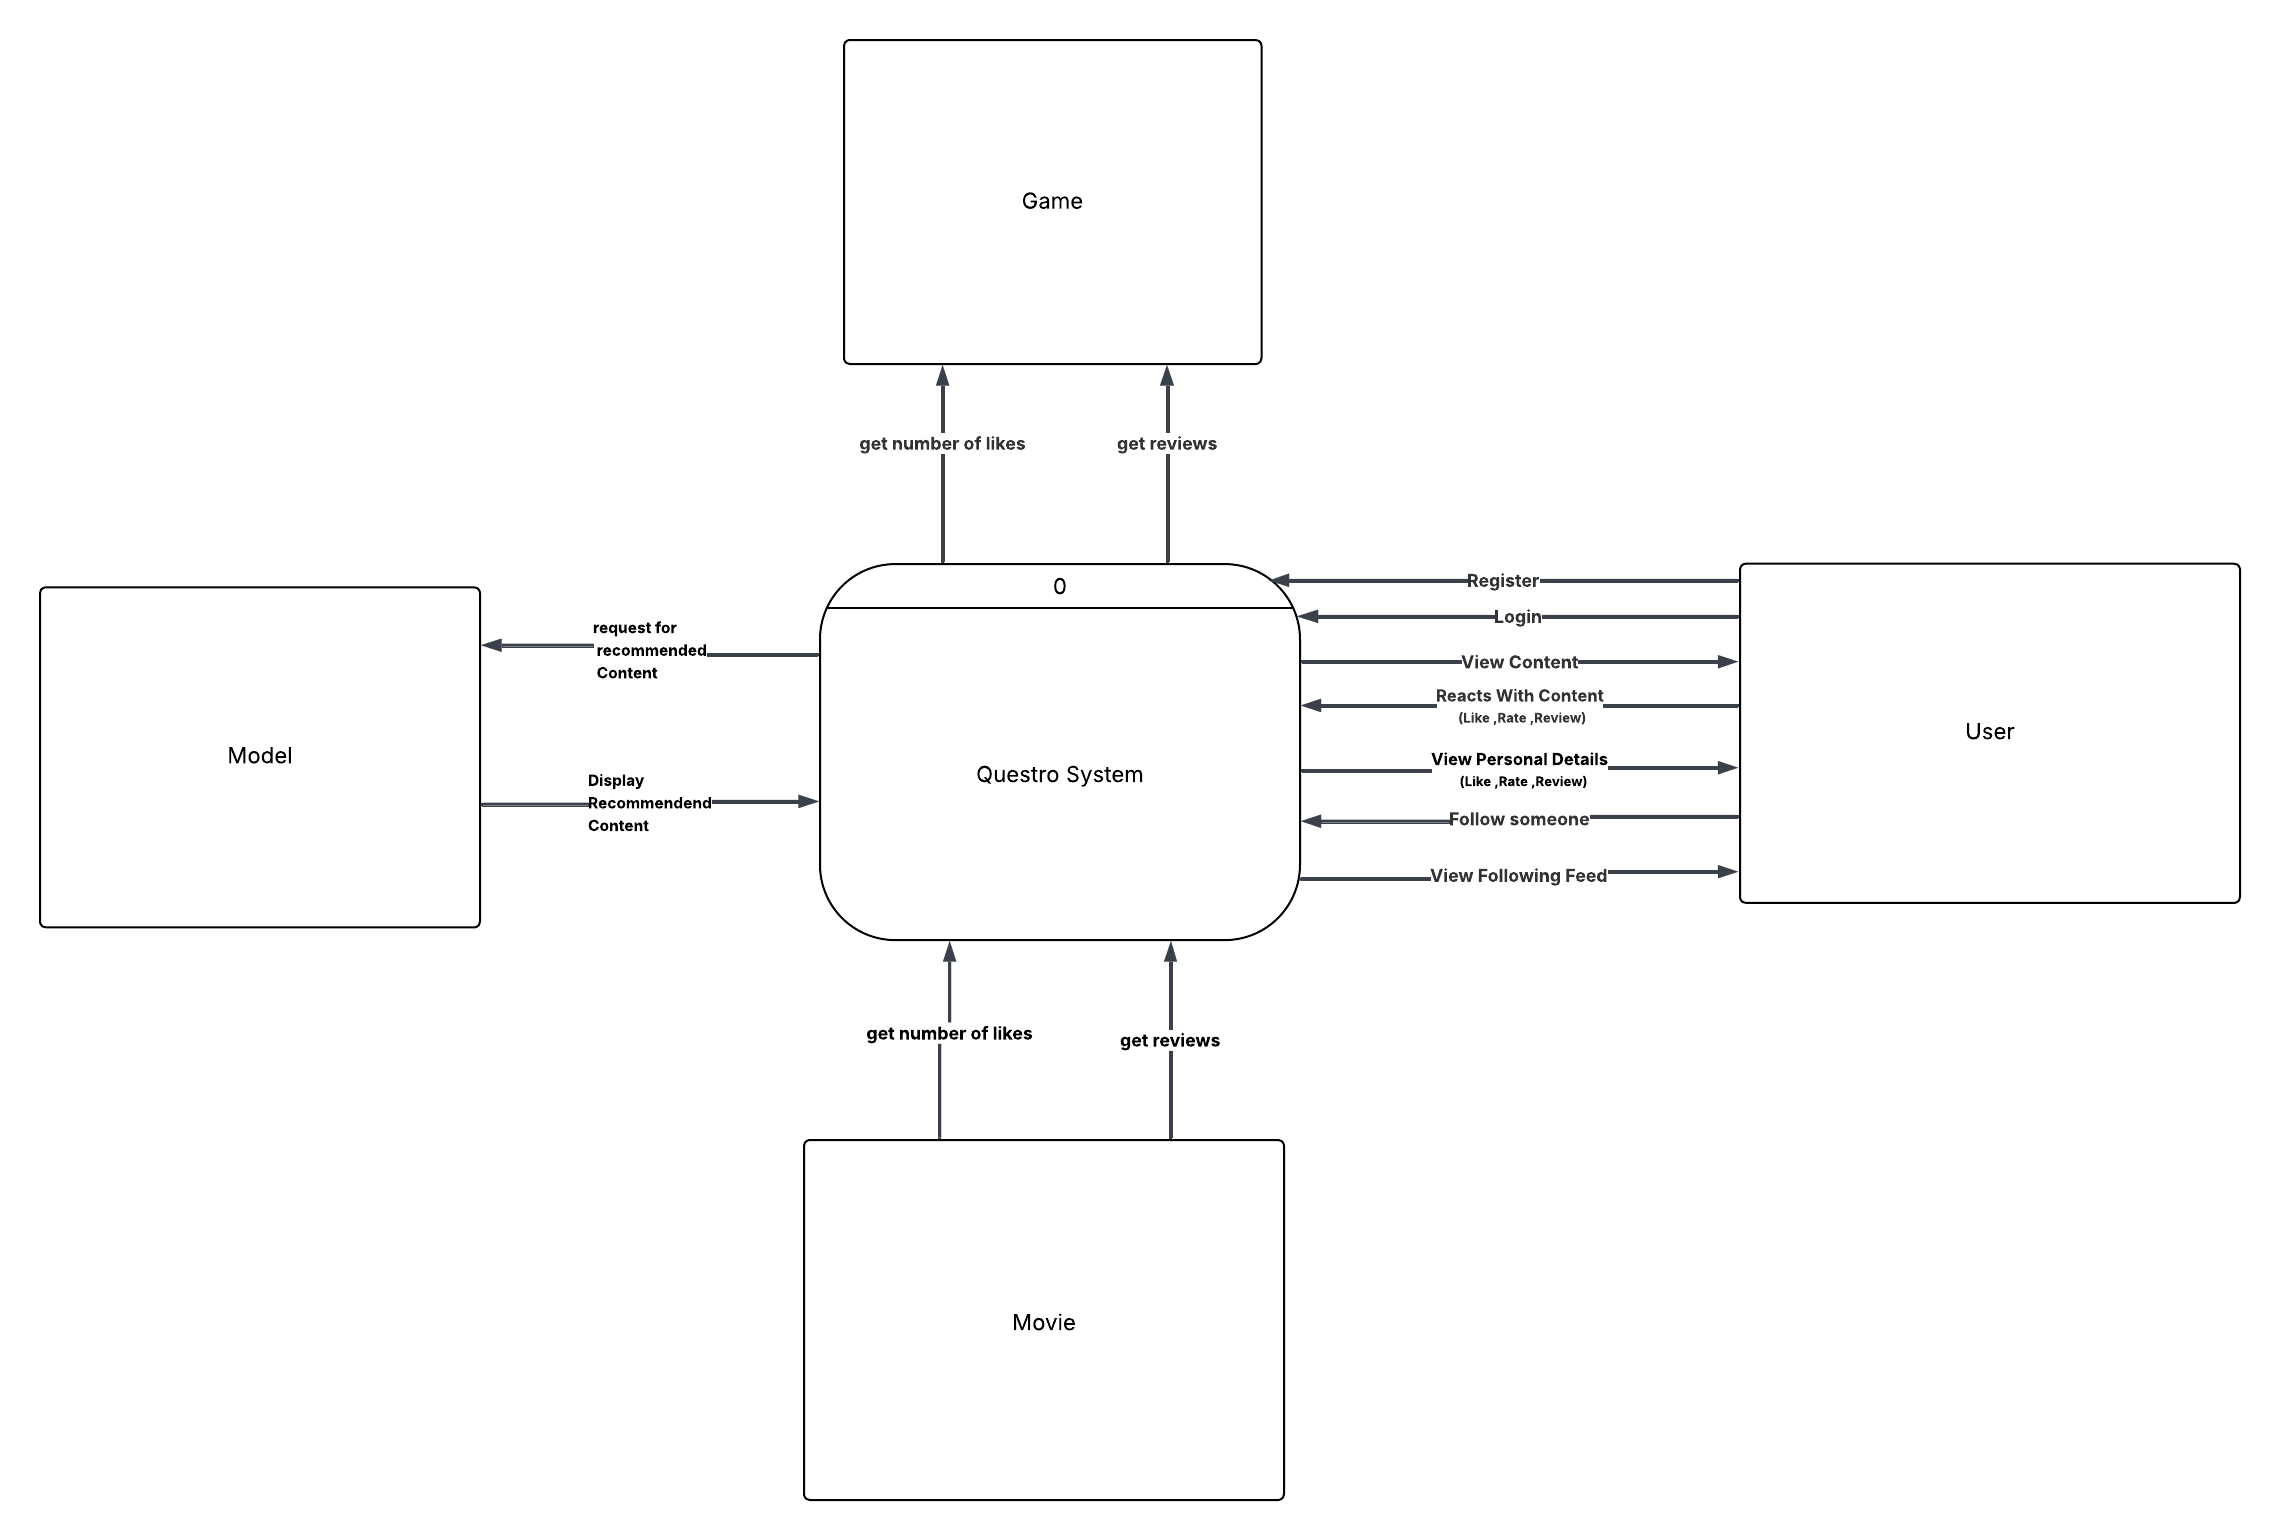
\includegraphics[width=1.0\linewidth]{figures/diagram/Context.png}
    \caption{Context Diagram of the Integrated Recommendation System}
    \label{fig:context_diagram}
\end{sidewaysfigure}

\clearpage
\section{Data Flow Diagram (DFD)}
\label{sec:dfd}
The Data Flow Diagram (Figure \ref{fig:dfd}) provides a Level 1 decomposition of the Questro system, breaking down the central process into four distinct functional subsystems. This visualization tracks the movement of information packets—from user inputs to database storage and back to the interface—highlighting the transformation of data at each stage.

The architecture is partitioned into the following logical processes:

\begin{enumerate}
    \item \textbf{Auth System (Process 1.0):} Acting as the security gatekeeper, this module ingests raw credentials (email/password) and validates them against the \textit{User Database}. Upon success, it issues session tokens (JWT) that accompany all subsequent data requests, ensuring that only authorized actors can trigger downstream processes.
    
    \item \textbf{Content Service (Process 2.0):} This acts as the central data aggregator. It receives search queries and filtering parameters from the user, retrieves metadata from the \textit{Movies \& Games Cache}, and formats the results for display. Crucially, it routes detailed item attributes to the Recommendation Engine to support content-based filtering.
    
    \item \textbf{Social Service (Process 3.0):} This subsystem manages the dynamic "Social Graph." It processes interaction data—such as "Follow User," "Like Review," or "Share Playlist"—and updates the \textit{Social Interaction Logs}. It also queries these logs to build the user's news feed, populating it with activities from their network.
    
    \item \textbf{Recommendation Engine (Process 4.0):} The computational core of the platform. It subscribes to the \textit{User Activity History} (clicks, ratings, time spent). Periodically or on-demand, it processes this historical data through hybrid algorithms to generate a ranked list of \textit{Predicted Item IDs}, which are then sent back to the Content Service for rendering.
\end{enumerate}

\begin{sidewaysfigure}
    \centering
    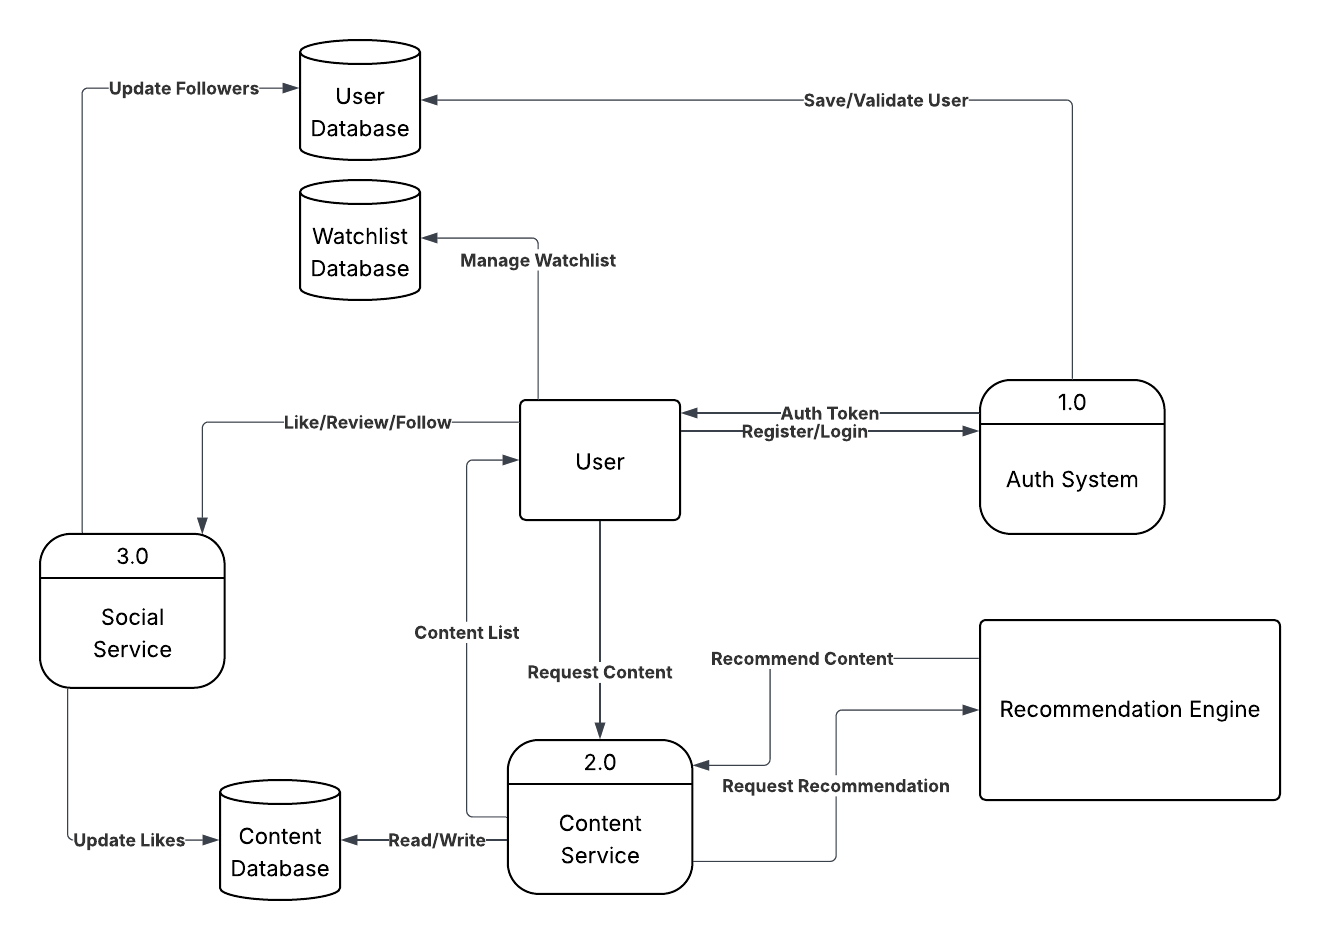
\includegraphics[width=1.0\linewidth]{figures/diagram/DFD.png}
    \caption{Level 1 Data Flow Diagram (DFD)}
    \label{fig:dfd}
\end{sidewaysfigure}

\clearpage
\section{Class Diagram}
\label{sec:class_diagram}
The Class Diagram (Figure \ref{fig:class_diagram}) depicts the static object-oriented structure of the backend application, serving as the blueprint for the system's code implementation. While the ERD focuses on data storage, this diagram illustrates the classes, attributes, methods, and the relationships (inheritance, association, and composition) that govern the runtime logic.

The architecture follows a modular design pattern, primarily categorized into three layers:

\begin{itemize}
    \item \textbf{Entity Layer (Data Models):} At the core is the \texttt{User} class, which aggregates personal details, preferences, and authentication credentials. The system utilizes polymorphism for content management through an abstract base class \texttt{MediaItem}. Both \texttt{Movie} and \texttt{Game} classes inherit from \texttt{MediaItem}, sharing common attributes like \textit{Title}, \textit{ReleaseDate}, and \textit{GlobalRating}, while encapsulating domain-specific attributes (e.g., \textit{Director} for movies, \textit{Publisher} for games).

    \item \textbf{Controller Layer (Business Logic):} The \texttt{RecommendationController} acts as the central orchestrator. It does not store data but instead calls methods from the Model layer to fetch user vectors, sends them to the ML engine, and returns a list of \texttt{MediaItem} objects. Similarly, the \texttt{AuthController} handles secure login sessions and token validation.

    \item \textbf{Managerial Layer (Social \& Interaction):} The \texttt{SocialManager} class handles complex graph operations. It manages lists of \texttt{Follower} and \texttt{Following} associations and calculates friendship metrics. Additionally, the \texttt{ReviewSystem} class links specific \texttt{User} instances to \texttt{MediaItem} instances, embedding sentiment analysis scores within the review object.
\end{itemize}

This structure ensures high cohesion and low coupling, allowing developers to update the recommendation algorithms (Strategy Pattern) without affecting the core data models.

\begin{sidewaysfigure}
    \centering
    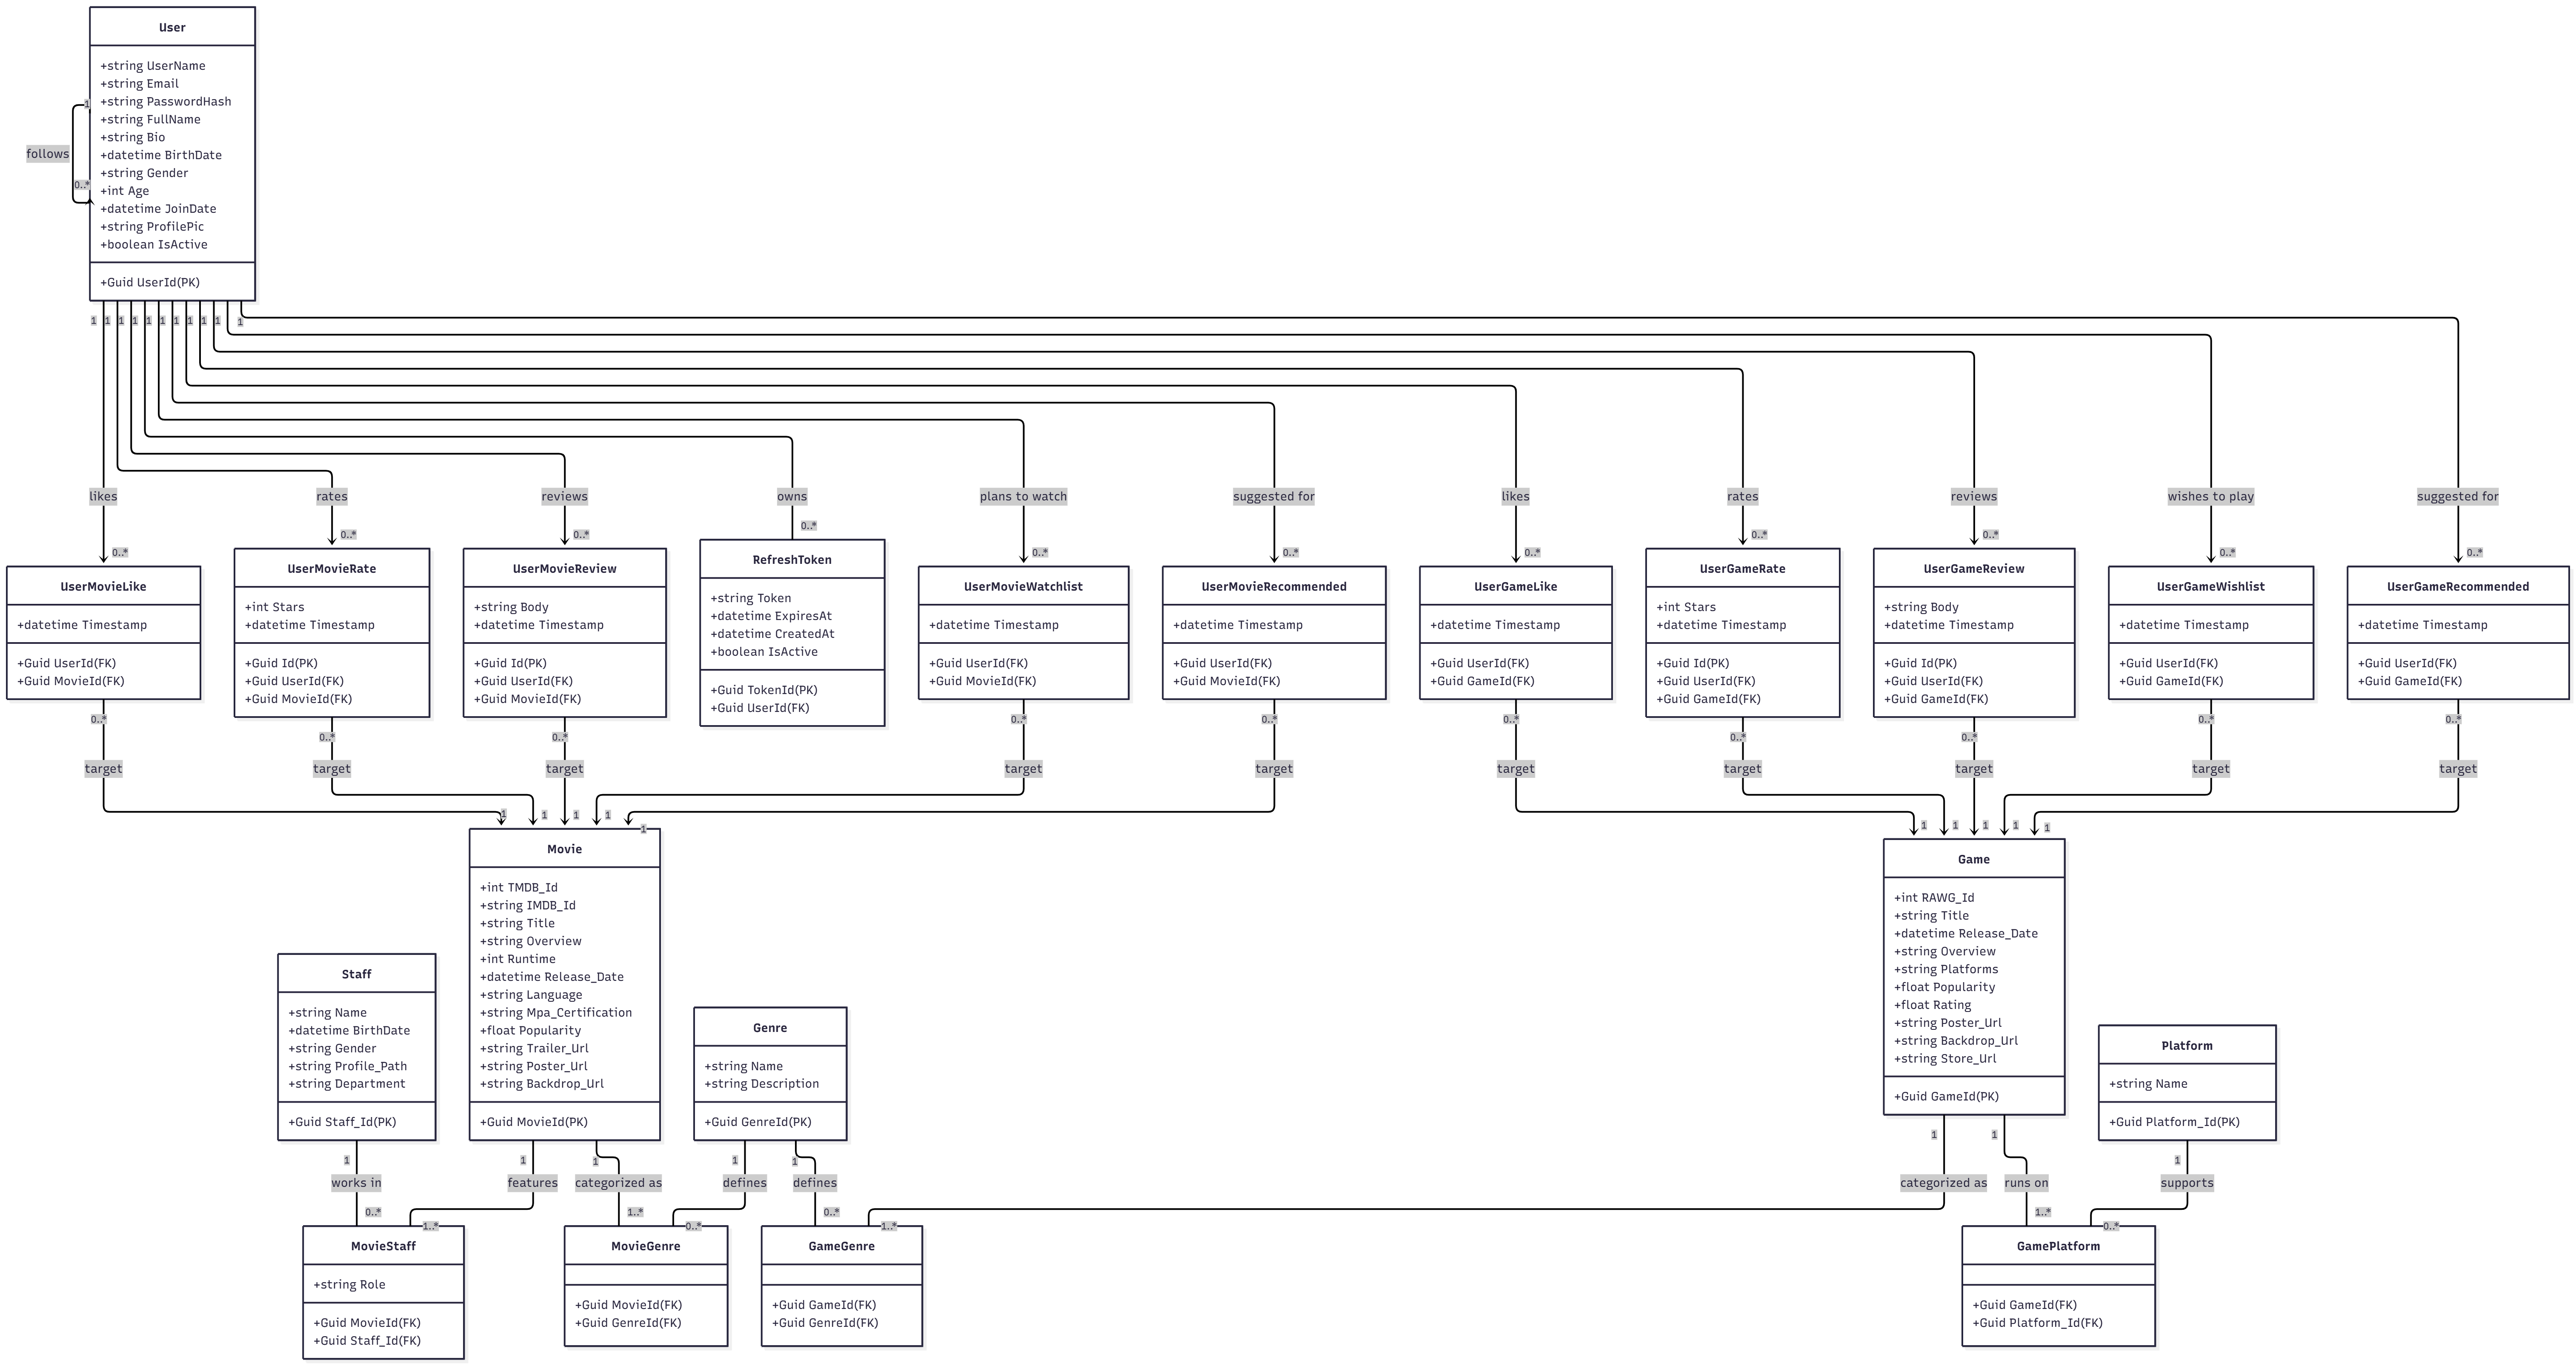
\includegraphics[width=1.0\linewidth]{figures/diagram/Class.png} 
    \caption{System Class Diagram}
    \label{fig:class_diagram}
\end{sidewaysfigure}

\clearpage

\section{Entity-Relationship (ER) Diagram}
\label{sec:erd}
The Entity-Relationship (ER) Diagram (Figure \ref{fig:er_diagram}) illustrates the logical data structure of the Questro backend, designed to maintain data integrity and optimize query performance. The schema follows the principles of Third Normal Form (3NF) to minimize redundancy and prevent update anomalies.

Given the heterogeneous nature of the content (Movies vs. Games), the database design adopts a modular approach centered around the following key areas:

\begin{itemize}
    \item \textbf{The Central User Entity:} The \texttt{User} table acts as the nucleus of the schema. It stores authentication credentials (hashed passwords, email) and profile metadata. Crucially, it serves as the primary key for foreign key relationships in all interaction tables, linking a single identity to diverse activities across both entertainment domains.

    \item \textbf{Domain-Specific Content Handling:} To address the distinct attributes of the two media types, the schema bifurcates into:
    \begin{itemize}
        \item \textbf{Movie Domain:} Includes tables for \texttt{Movies}, \texttt{Cast}, \texttt{Crew}, and \texttt{ProductionCompanies}. It manages specific attributes such as \textit{Runtime}, \textit{Director}, and \textit{BoxOffice}.
        \item \textbf{Game Domain:} Includes tables for \texttt{Games}, \texttt{Developers}, \texttt{Publishers}, and \texttt{Platforms}. It handles attributes unique to gaming, such as \textit{AveragePlaytime} and \textit{MetacriticScore}.
    \end{itemize}

    \item \textbf{Interaction \& Association (Many-to-Many):} The diagram highlights the use of junction tables (associative entities) to manage many-to-many relationships. For example, the \texttt{User\_Review} and \texttt{User\_Rating} tables link users to content items while storing additional attributes like timestamps and sentiment scores. Similarly, the social graph is modeled through self-referencing relationships on the User table to represent \textit{Followers} and \textit{Following}.
\end{itemize}

This structured approach ensures that the system can efficiently execute complex join queries required for the hybrid recommendation engine.

\begin{sidewaysfigure}
    \centering
    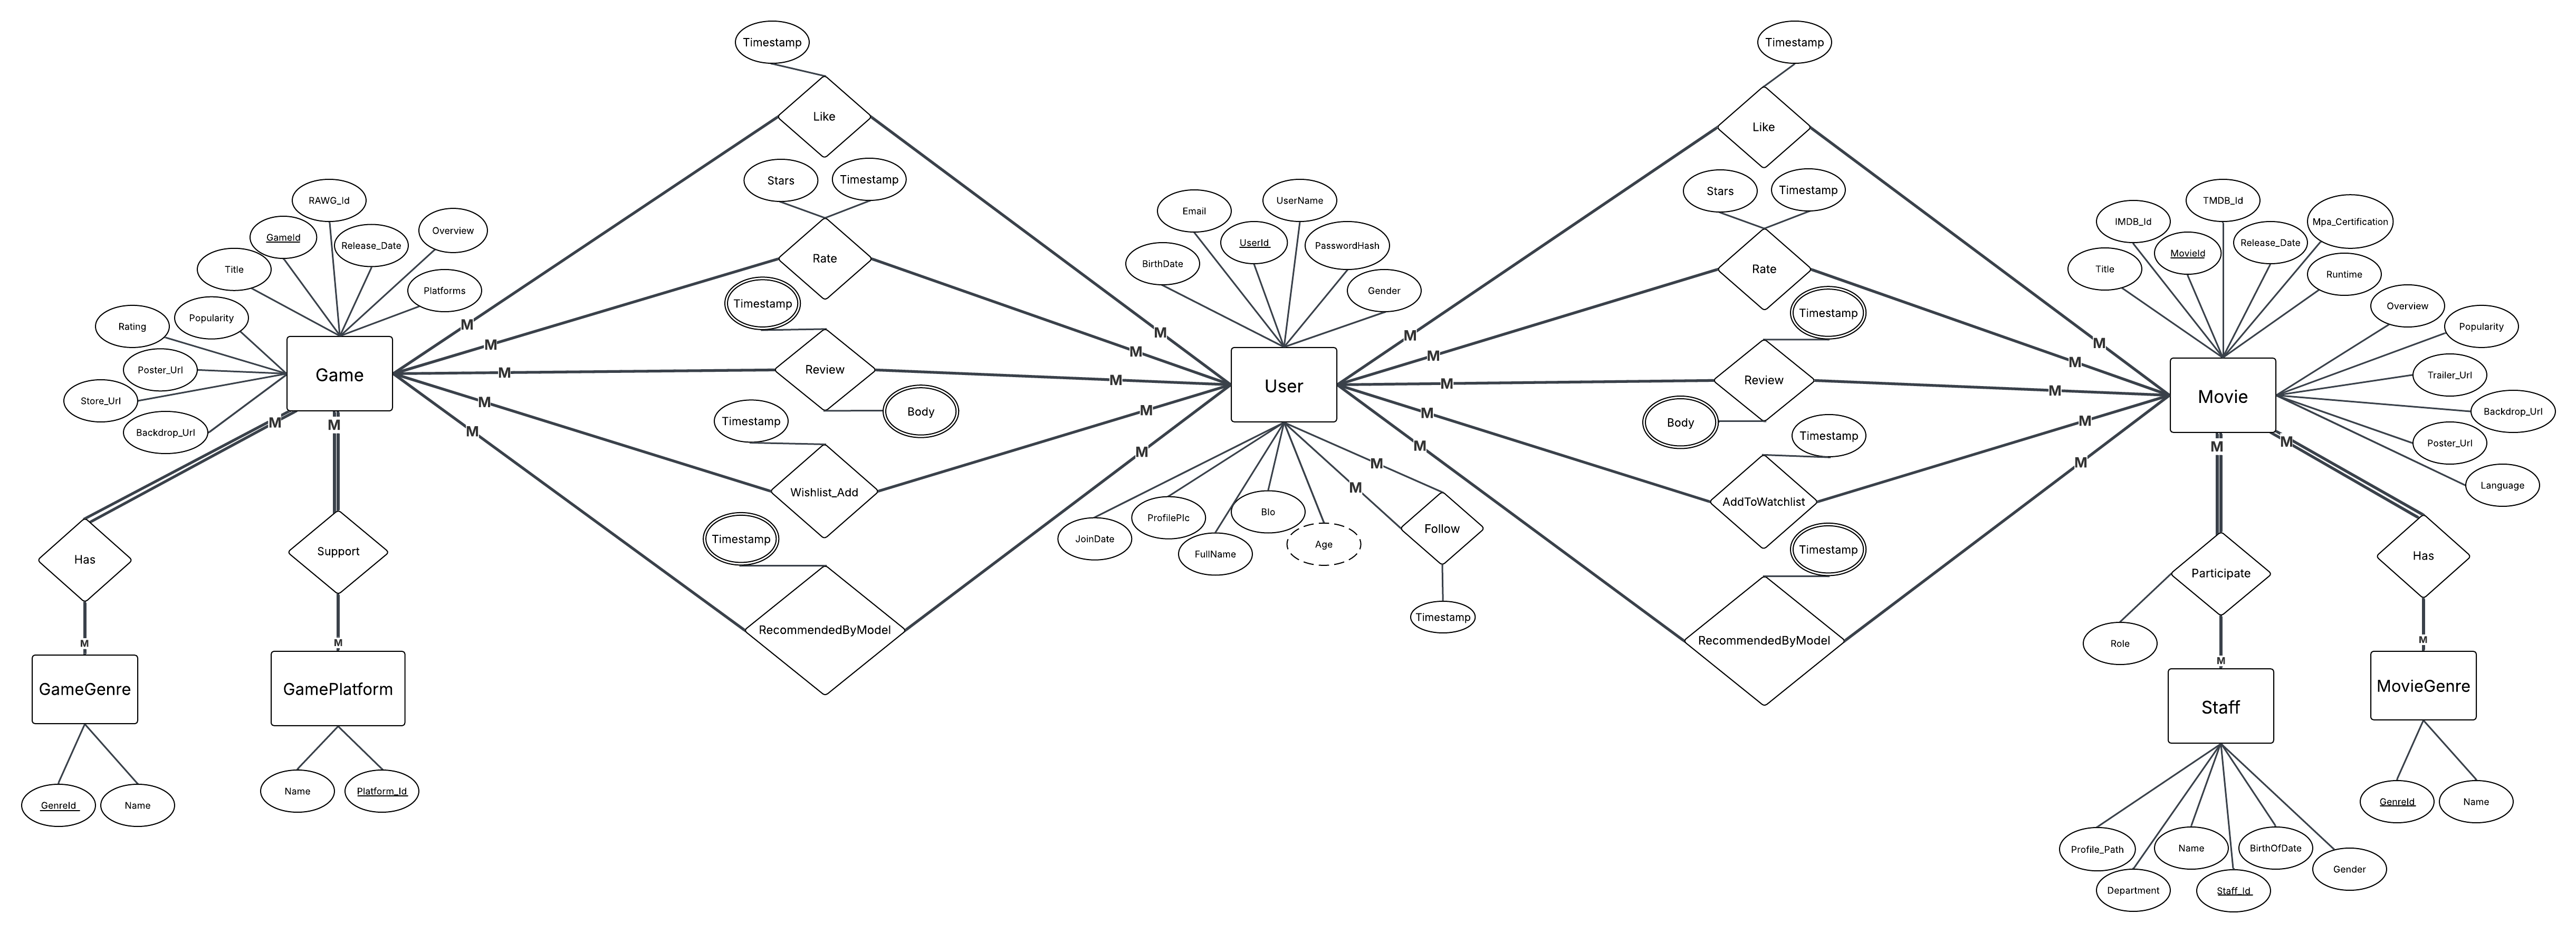
\includegraphics[width=1.0\linewidth]{figures/diagram/ERD.png}
    \caption{Entity-Relationship (ER) Diagram}
    \label{fig:er_diagram}
\end{sidewaysfigure}

\clearpage

\section{Sequence Diagrams}
This section details the dynamic behavior of the system, visualizing the step-by-step message passing between Actors, the System Backend, the Database, and the ML Models.

\subsection{Authentication \& Onboarding}
The entry point for all users involves secure validation and initial profile building.
\textbf{Workflow:} As shown in Figure \ref{fig:seq_signup}, the registration process handles the "Cold Start" problem. Immediately after account creation, the user is presented with an \textit{Initiation Survey}. These initial preferences are fed directly to the Model to generate a "Day 1" recommendation list.

\begin{figure}[H]
    \centering
    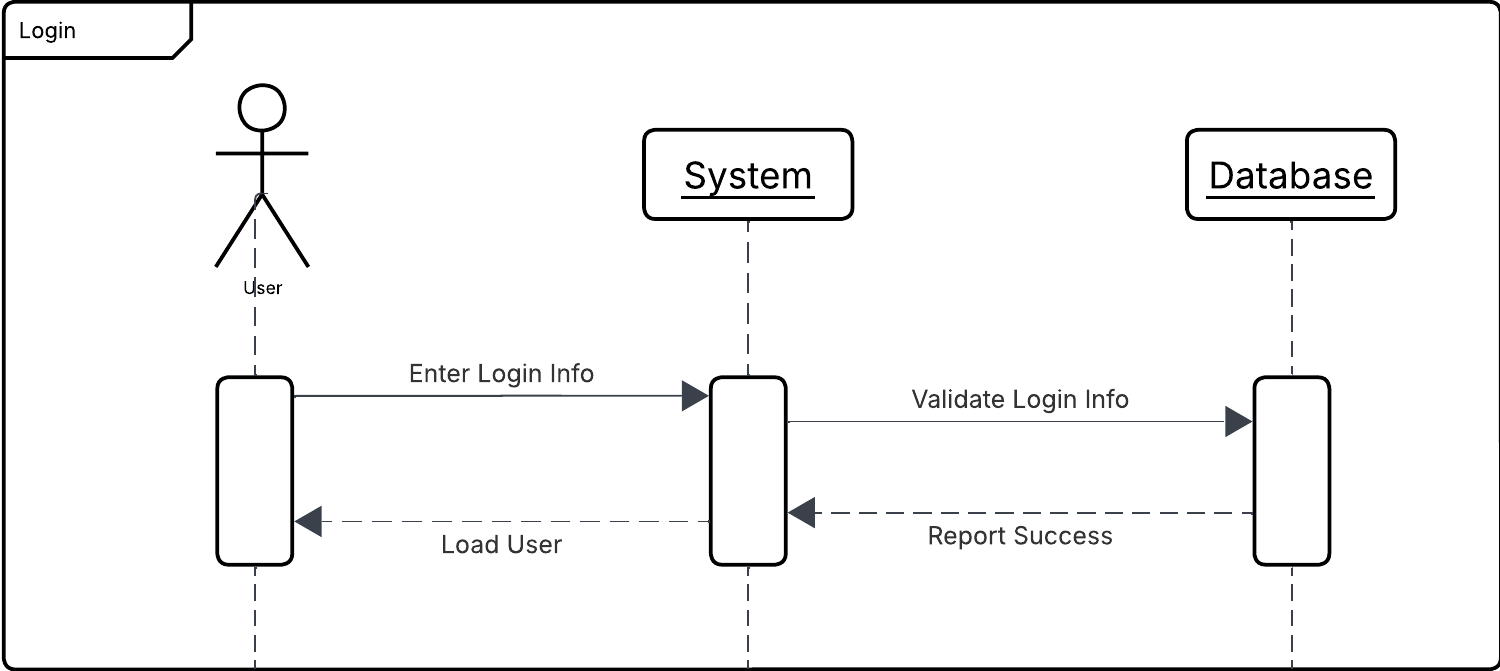
\includegraphics[width=1.0\linewidth]{figures/diagram/sequence/login.png}
    \caption{User Login Sequence}
    \label{fig:seq_login}
\end{figure}

\begin{figure}[H]
    \centering
    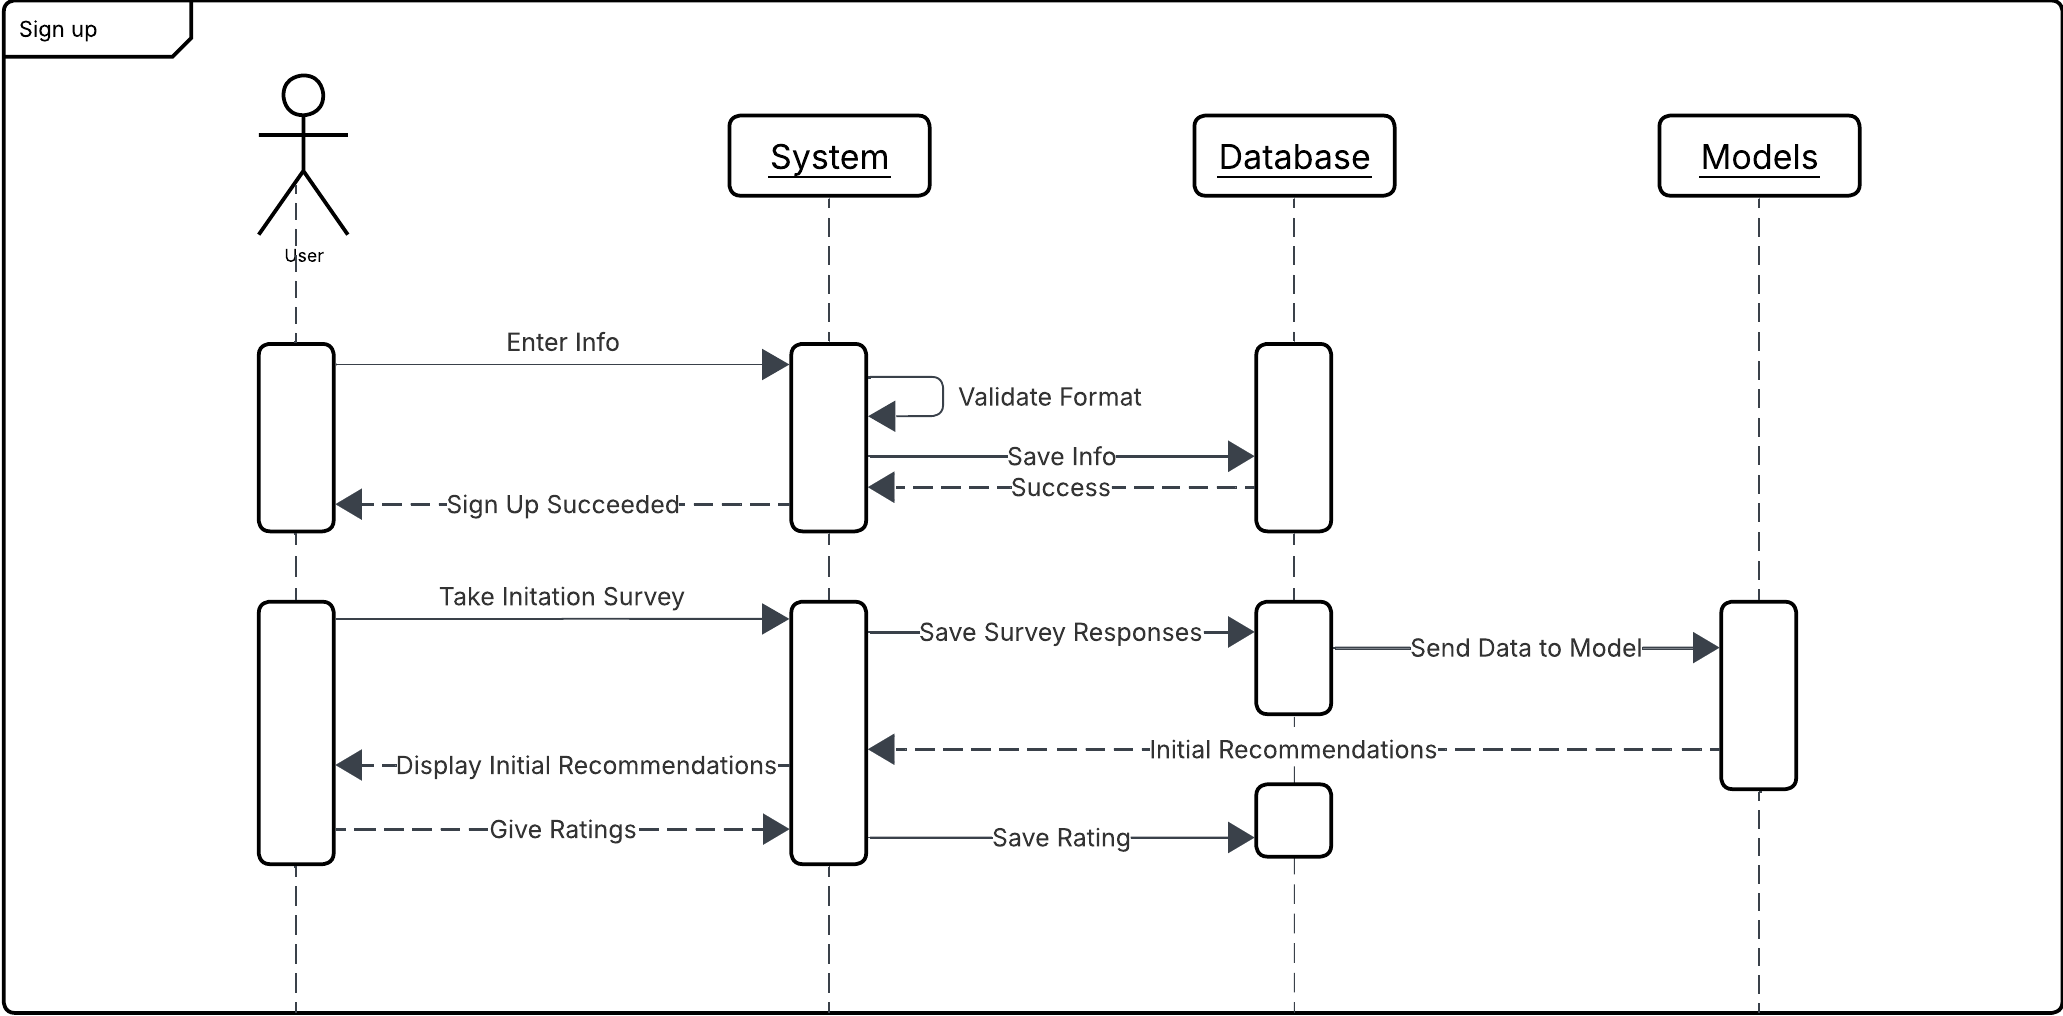
\includegraphics[width=1.0\linewidth]{figures/diagram/sequence/sign_up.png}
    \caption{Sign Up and Cold Start Handling}
    \label{fig:seq_signup}
\end{figure}


\subsection{Content Discovery Features}
Users have multiple methods to discover content, ranging from deliberate searches to randomized suggestions.

The \textbf{Surprise Me} feature (Figure \ref{fig:seq_surprise}) breaks the "filter bubble." When triggered, the system bypasses standard history-based weighting and requests a randomized, high-entropy item queue from the database, offering users a chance to explore genres they typically ignore.

\begin{figure}[H]
    \centering
    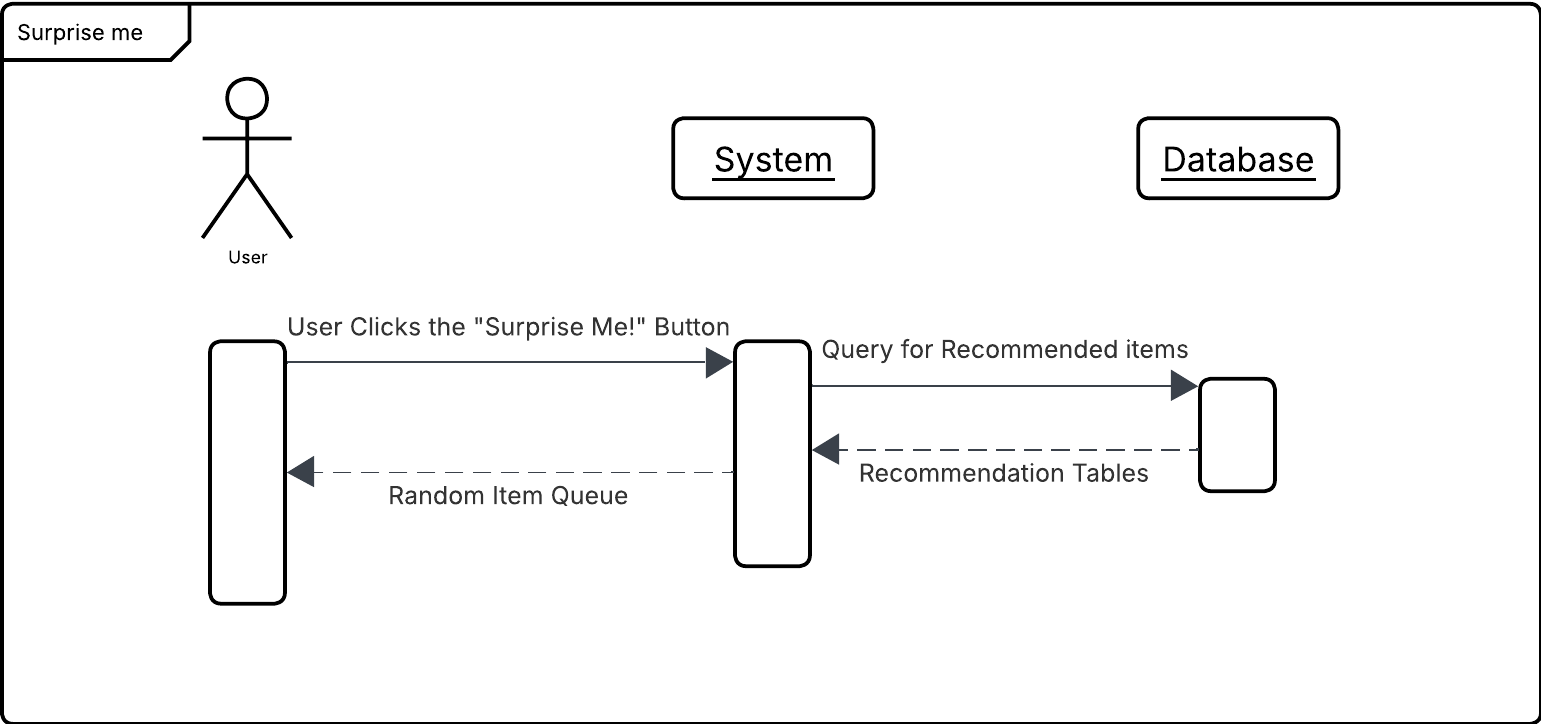
\includegraphics[width=1.0\linewidth]{figures/diagram/sequence/surprise_me.png}
    \caption{Surprise Me Algorithm Sequence}
    \label{fig:seq_surprise}
\end{figure}

Figure \ref{fig:seq_favorites} demonstrates the implicit feedback loop. Adding an item to favorites is not just a database storage action; it triggers a specialized event sent to the \textbf{Model}, which immediately re-weighs the user's preference vector for future sessions.

\begin{figure}[H]
    \centering
    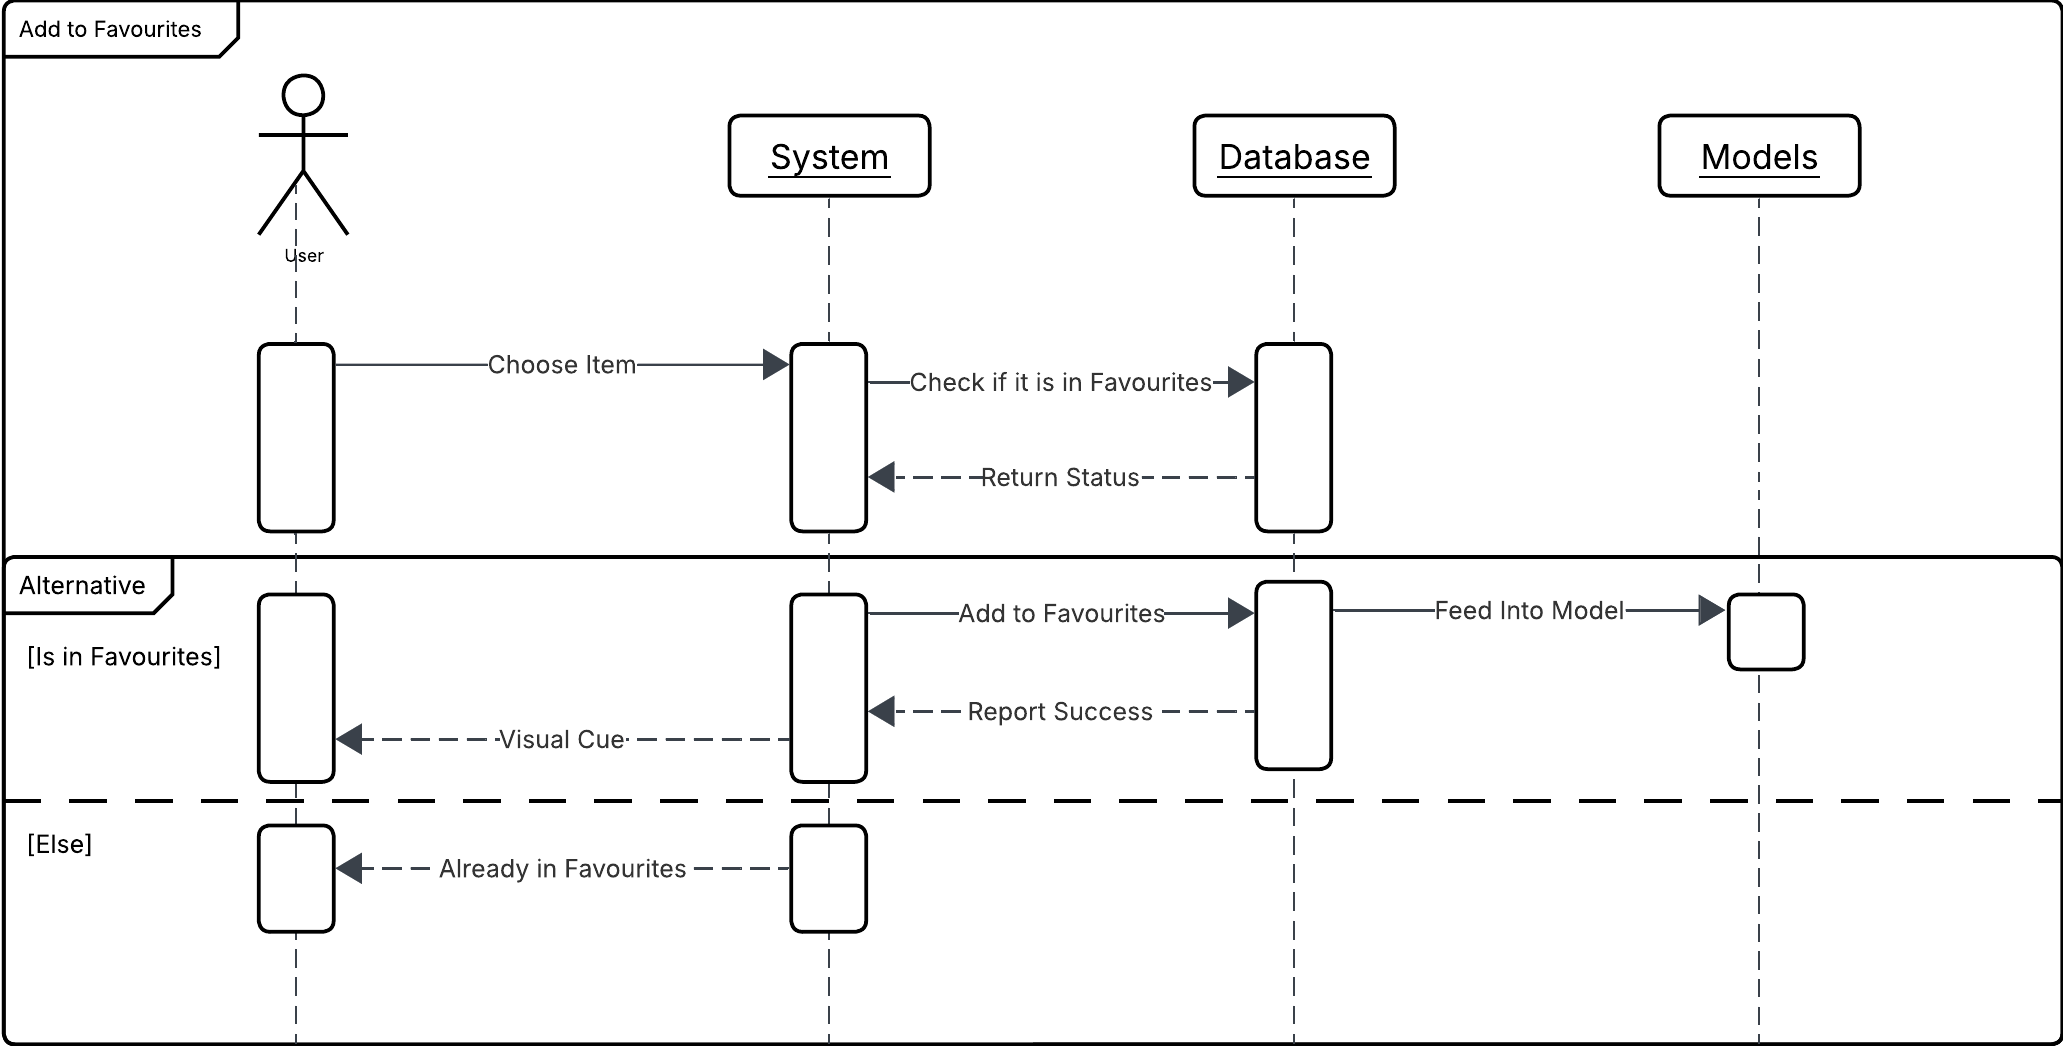
\includegraphics[width=1.0\linewidth]{figures/diagram/sequence/add_to_favorites.png}
    \caption{Add to Favorites \& Model Feedback Loop}
    \label{fig:seq_favorites}
\end{figure}


\subsection{Social Interaction \& Gamification}
Questro includes robust social features to increase user retention.

The review process (Figure \ref{fig:seq_review}) is enhanced by Natural Language Processing (NLP). When a review is submitted, it is passed to a Sentiment Analysis model. The resulting sentiment score adjusts the weight of that item in the user's profile (e.g., a negative review decreases recommendation likelihood for similar items).

\begin{figure}[H]
    \centering
    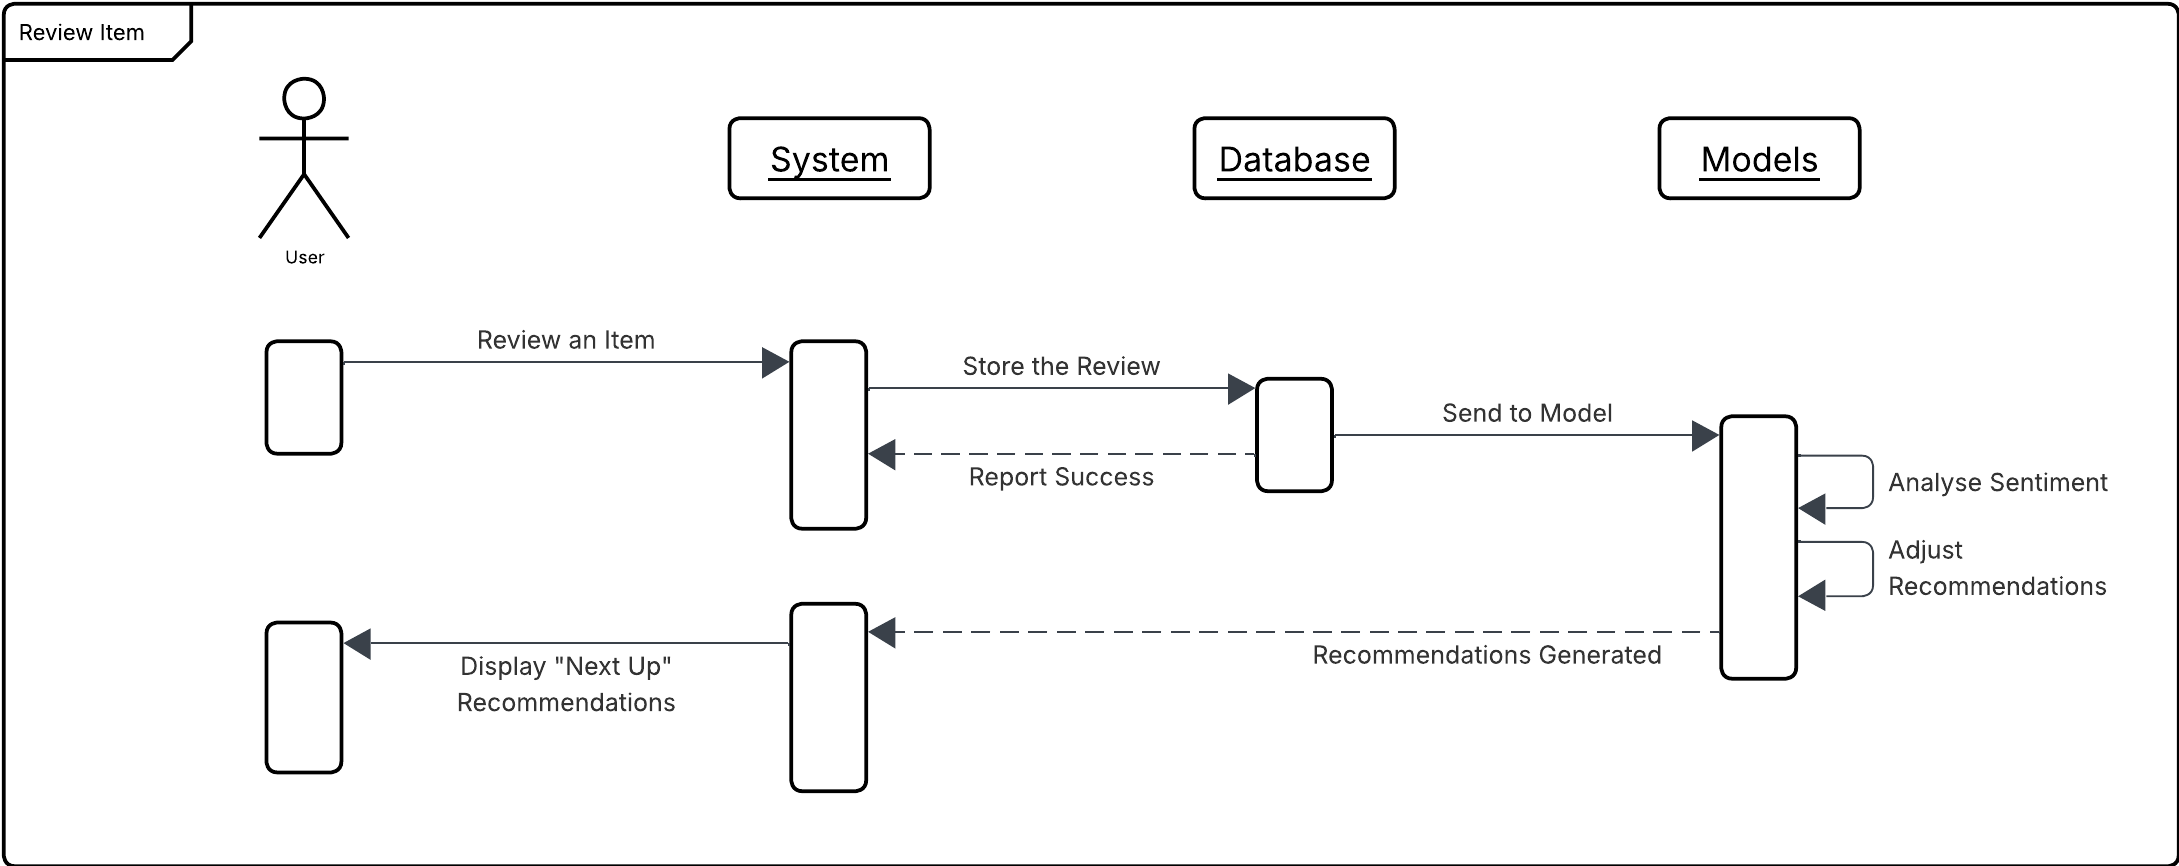
\includegraphics[width=1.0\linewidth]{figures/diagram/sequence/review_item.png}
    \caption{Review Submission with Sentiment Analysis}
    \label{fig:seq_review}
\end{figure}

\begin{figure}[H]
    \centering
    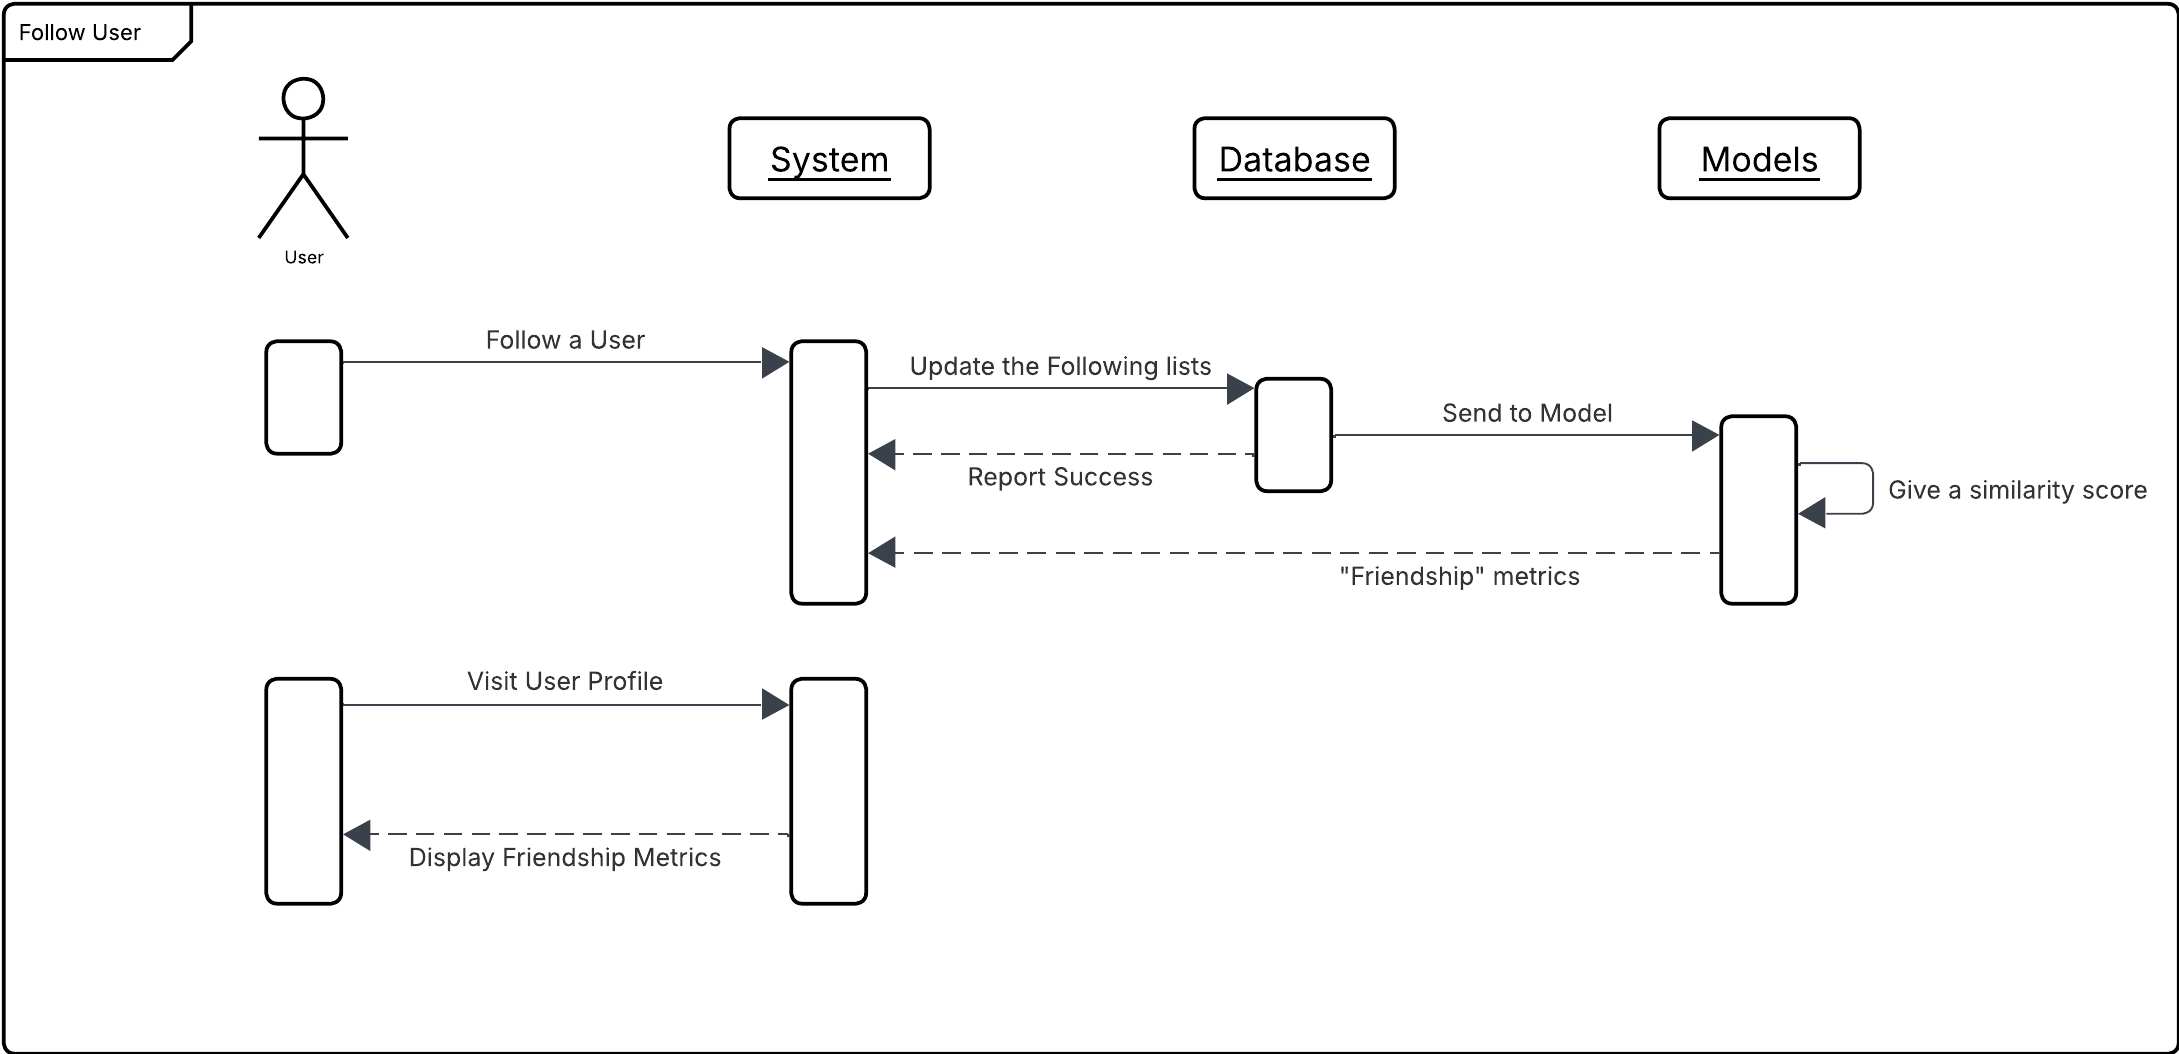
\includegraphics[width=1.0\linewidth]{figures/diagram/sequence/follow_user.png}
    \caption{Social Following \& Friendship Metrics}
    \label{fig:seq_follow}
\end{figure}

To encourage engagement, the system uses a \textbf{Badge System} (Figure \ref{fig:seq_badges}). The backend validates user actions (e.g., "Rated 50 Movies") and awards badges. If an action is found to be illegitimate, the system can revoke the badge dynamically.

\begin{figure}[H]
    \centering
    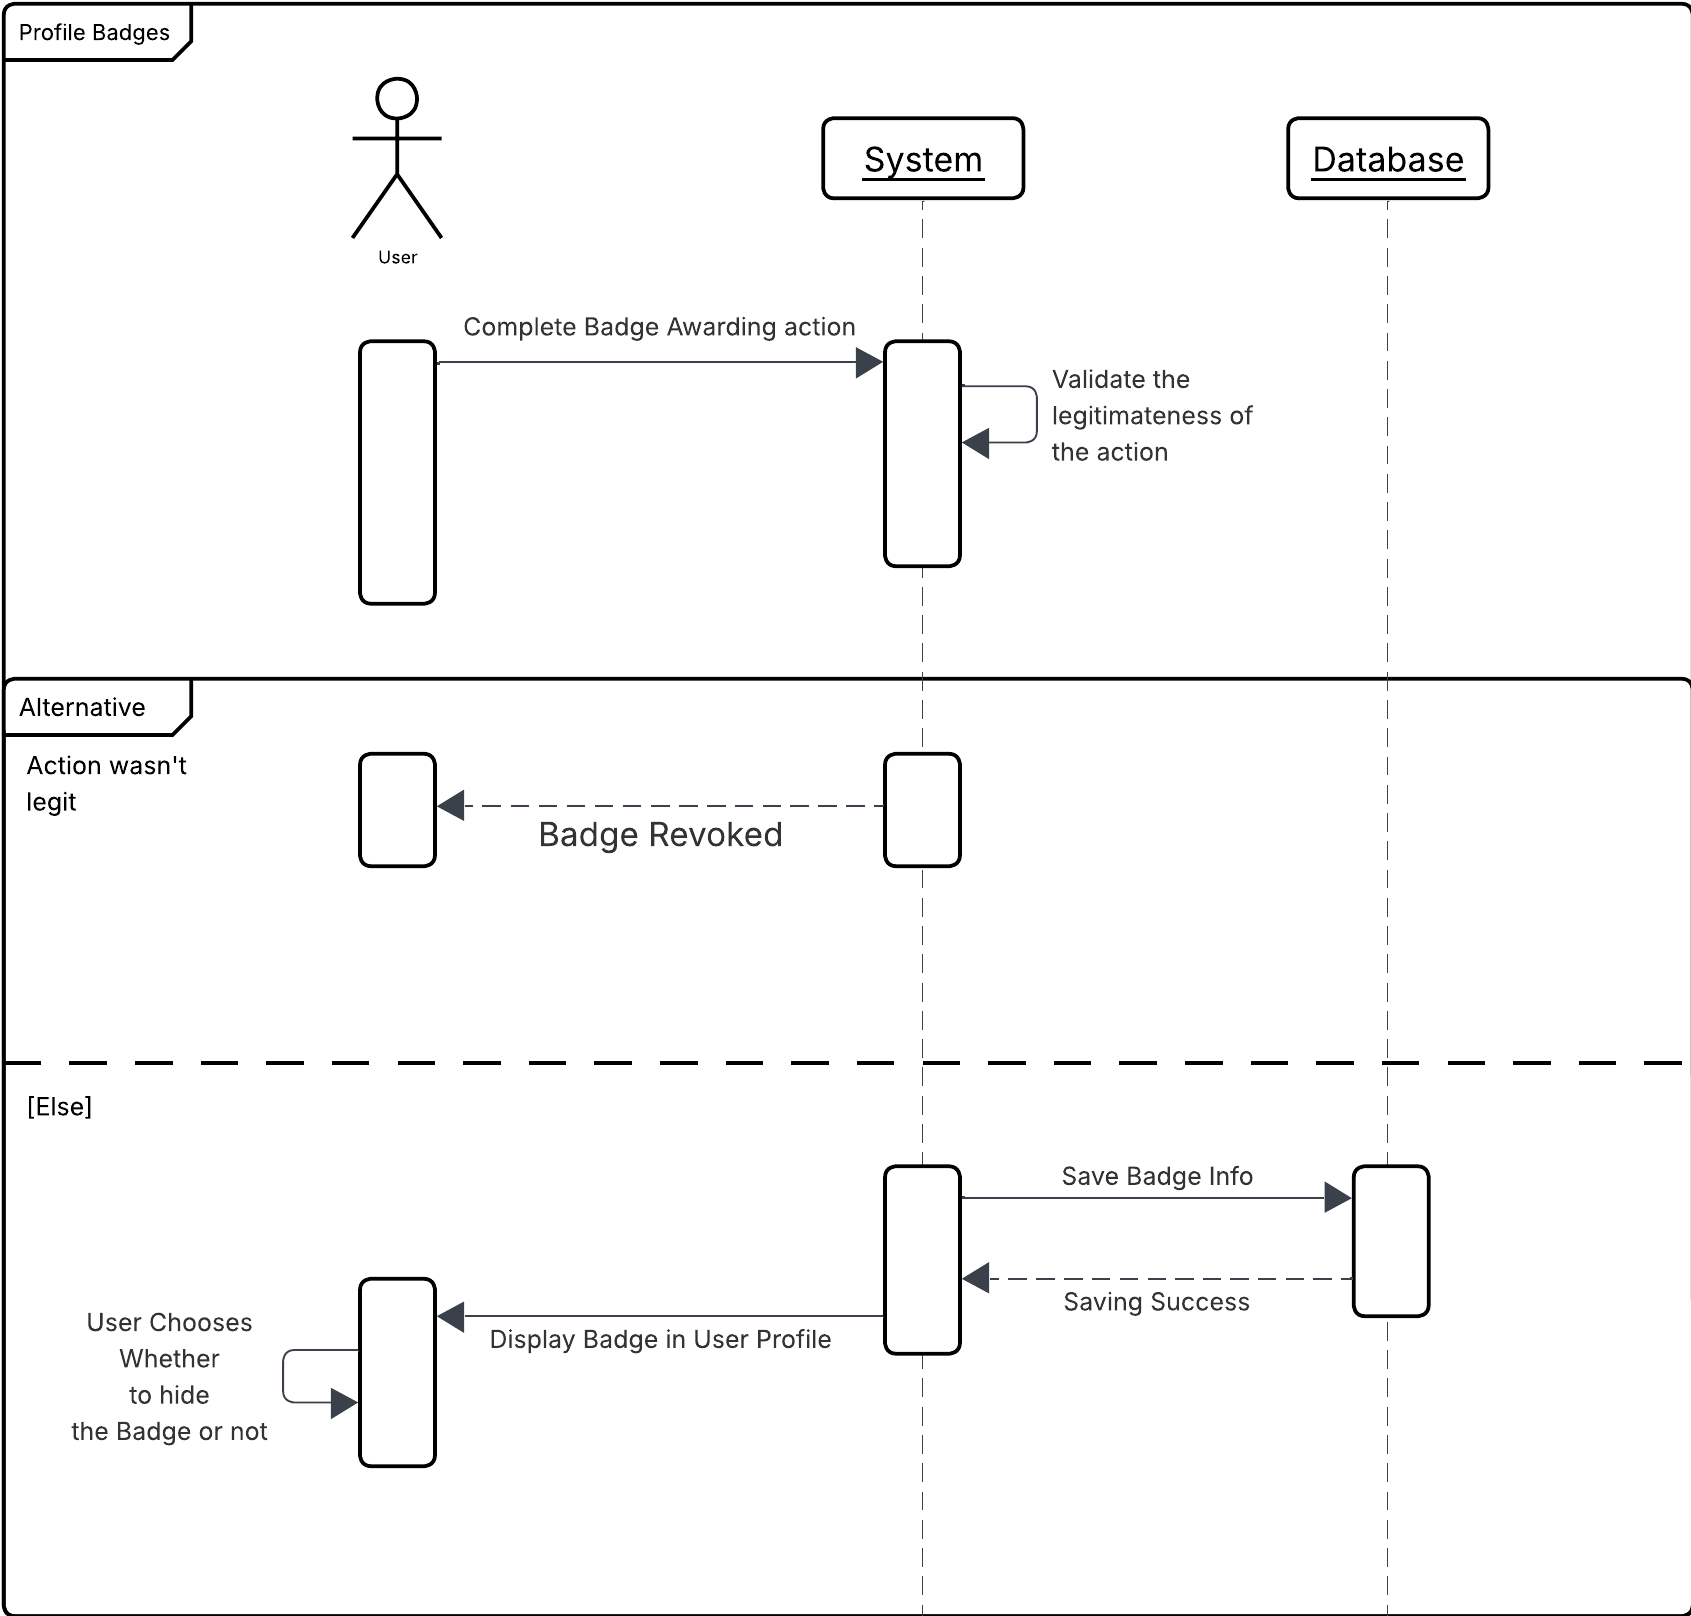
\includegraphics[width=1.0\linewidth]{figures/diagram/sequence/profile_badges.png}
    \caption{Gamification: Badge Awarding System}
    \label{fig:seq_badges}
\end{figure}

\subsection{Privacy \& Parental Controls}
Given the diverse user base, safety and privacy are paramount.

\begin{figure}[H]
    \centering
    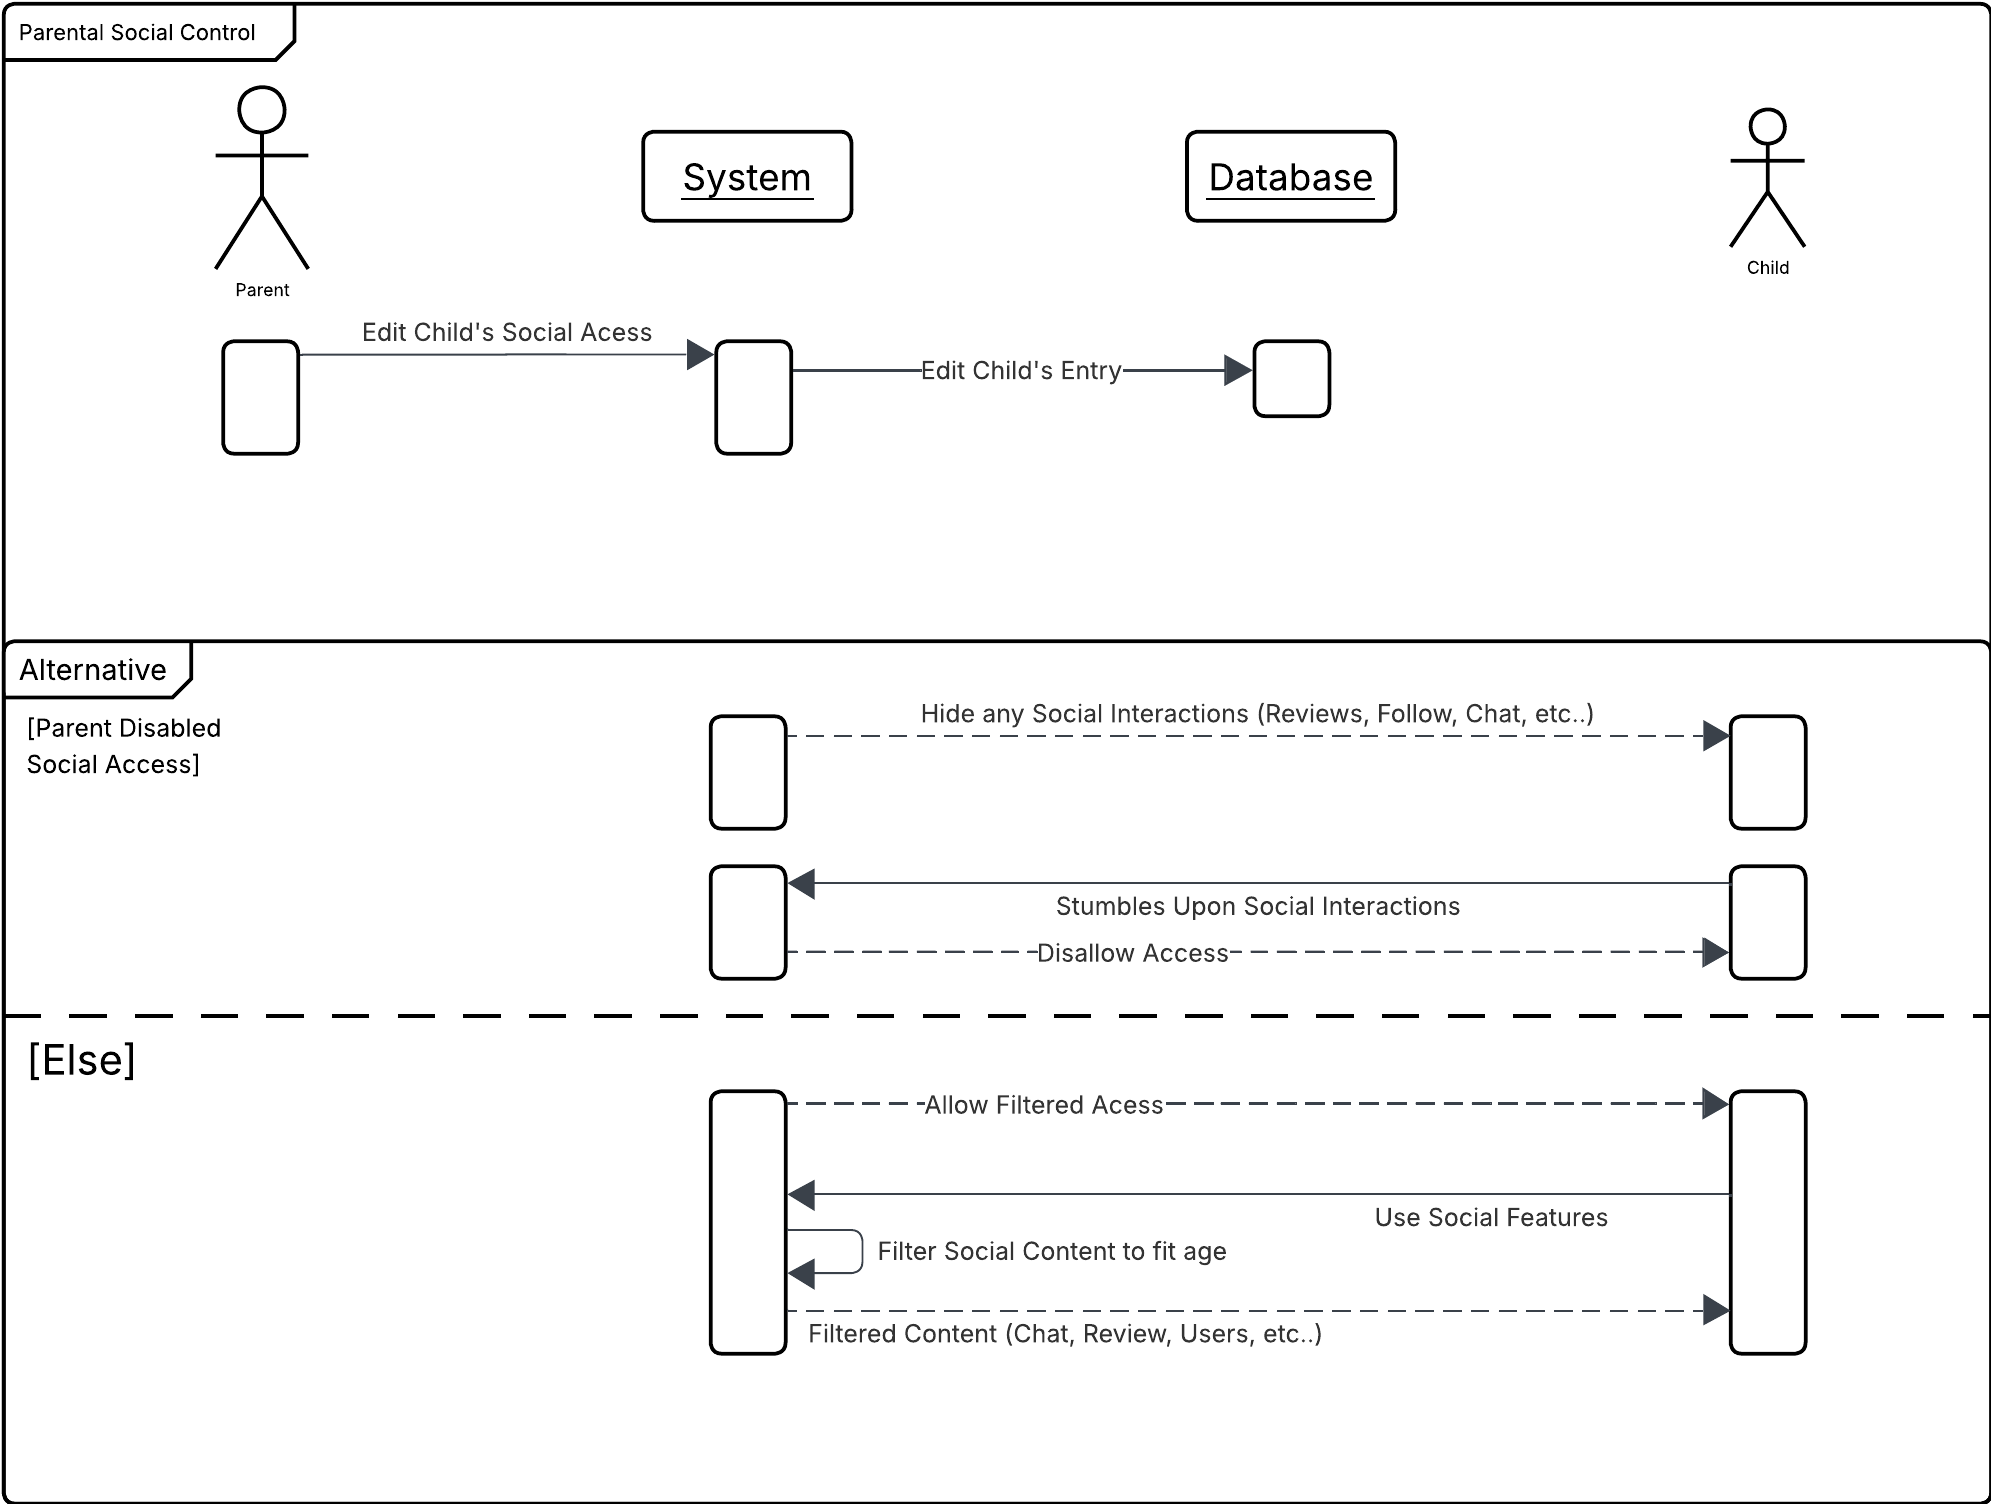
\includegraphics[width=1.0\linewidth]{figures/diagram/sequence/parental_control.png}
    \caption{Parental Control: Limiting Social Access}
    \label{fig:seq_parental_control}
\end{figure}

\begin{figure}[H]
    \centering
    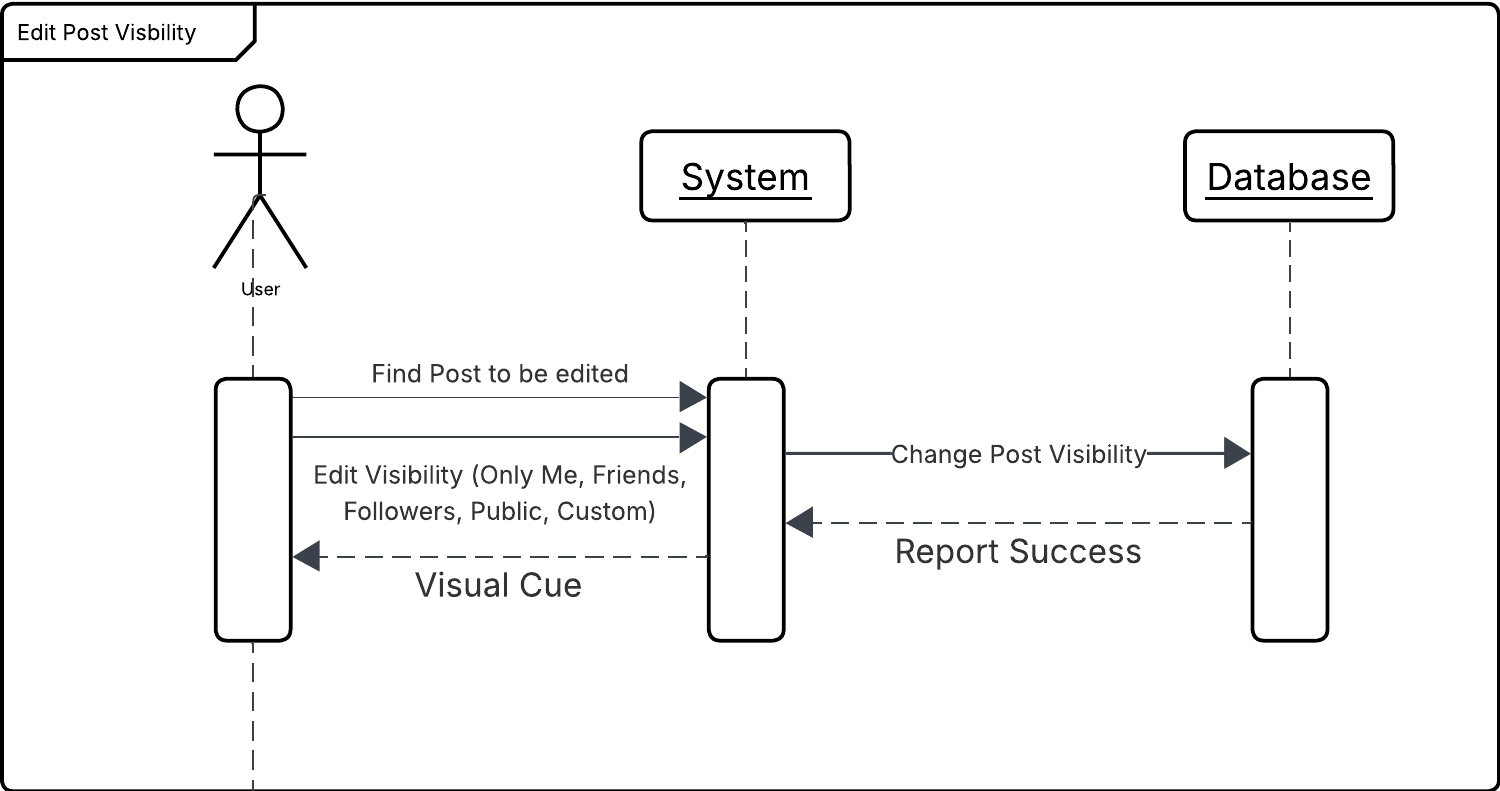
\includegraphics[width=1.0\linewidth]{figures/diagram/sequence/edit_post_visibility.png}
    \caption{Granular Privacy Settings for User Posts}
    \label{fig:seq_privacy}
\end{figure}

\newpage
\section{Use Case Scenarios}
The following use case scenarios describe various functionalities within the movie-game recommendation system.
\begin{table}[H]
    \centering
    \caption{Sign Up Sequence Scenario}
    \label{tab:signup}
    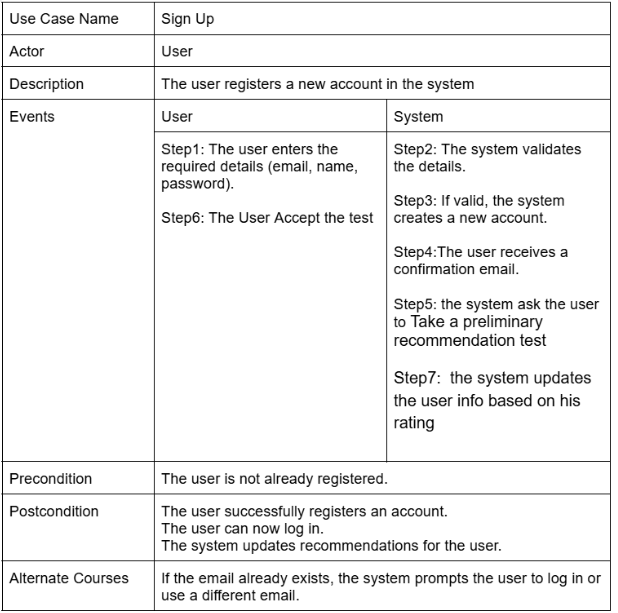
\includegraphics[width=\linewidth]{figures/diagram/Use Case Scenarios/Use Case Scenarios/Sign Up.png}
\end{table}

\begin{table}[H]
    \centering
    \caption{Log In Sequence Scenario}
    \label{tab:login}
    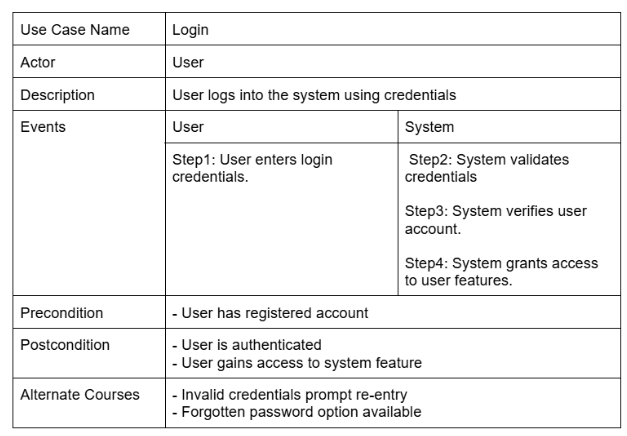
\includegraphics[width=\linewidth]{figures/diagram/Use Case Scenarios/Use Case Scenarios/Log In.png}
\end{table}

\begin{table}[H]
    \centering
    \caption{Recommend Item Scenario}
    \label{tab:recommend}
    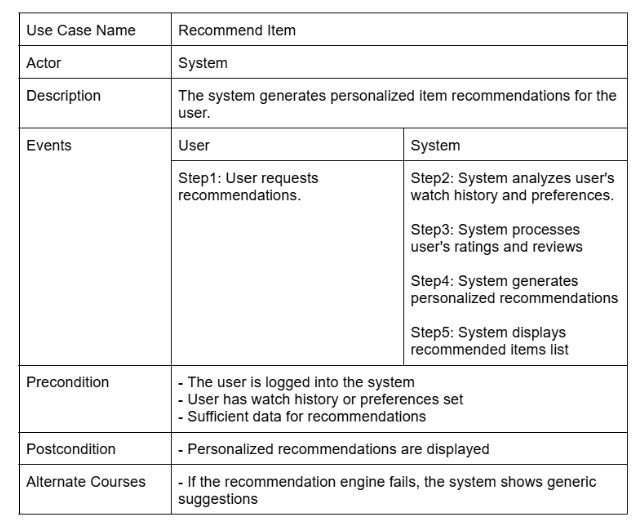
\includegraphics[width=\linewidth]{figures/diagram/Use Case Scenarios/Use Case Scenarios/RecommendItem.png}
\end{table}

\begin{table}[H]
    \centering
    \caption{View Available Movies Sequence Scenario}
    \label{tab:available-movies}
    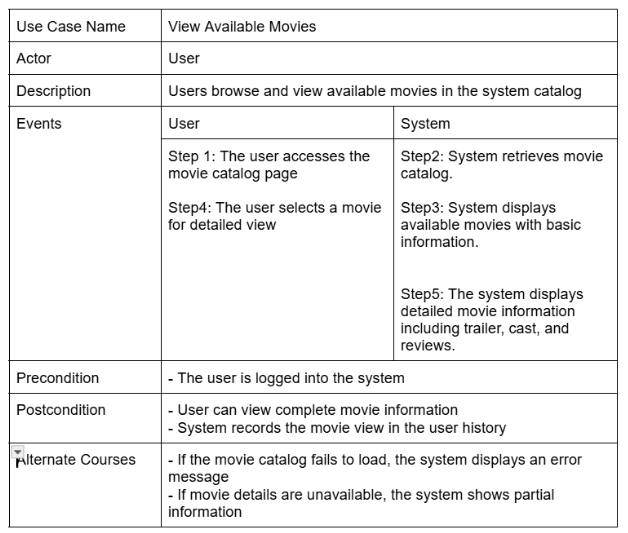
\includegraphics[width=\linewidth]{figures/diagram/Use Case Scenarios/Use Case Scenarios/AvilableMovies.png}
\end{table}

\begin{table}[H]
    \centering
    \caption{View Available Games Sequence Scenario}
    \label{tab:available-games}
    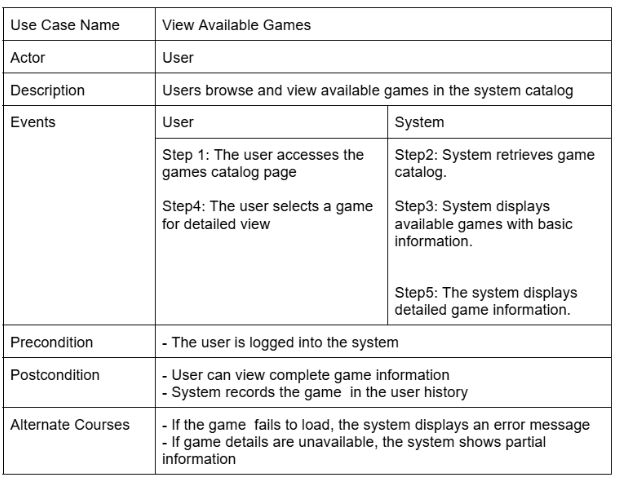
\includegraphics[width=\linewidth]{figures/diagram/Use Case Scenarios/Use Case Scenarios/AvilableGames.png}
\end{table}

\begin{table}[H]
    \centering
    \caption{Show Item Similarity List Sequence Scenario}
    \label{tab:item-similarity}
    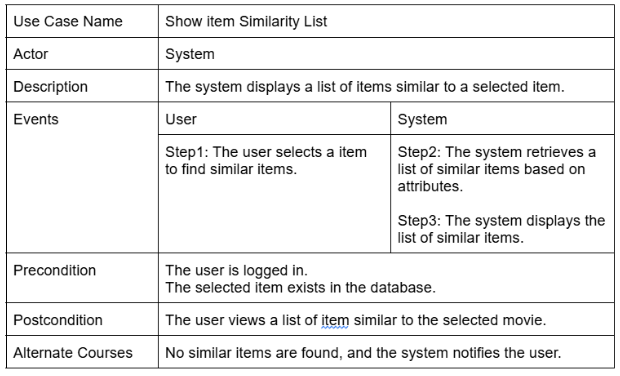
\includegraphics[width=\linewidth]{figures/diagram/Use Case Scenarios/Use Case Scenarios/itemSemilarity.png}
\end{table}

\begin{table}[H]
    \centering
    \caption{Likes Movie List Sequence Scenario}
    \label{tab:likes-movie}
    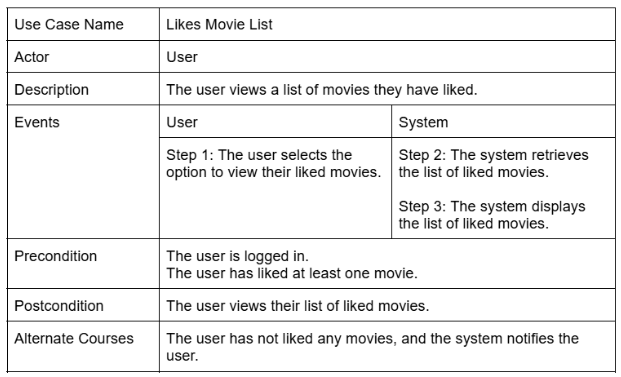
\includegraphics[width=\linewidth]{figures/diagram/Use Case Scenarios/Use Case Scenarios/LikesMovie.png}
\end{table}

\begin{table}[H]
    \centering
    \caption{Likes Game List Sequence Scenario}
    \label{tab:likes-game}
    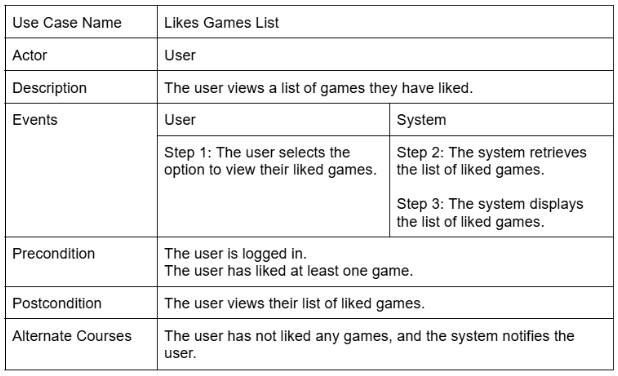
\includegraphics[width=\linewidth]{figures/diagram/Use Case Scenarios/Use Case Scenarios/LikesGameList.png}
\end{table}

\begin{table}[H]
    \centering
    \caption{Like/Unlike Item Sequence Scenario}
    \label{tab:like-unlike}
    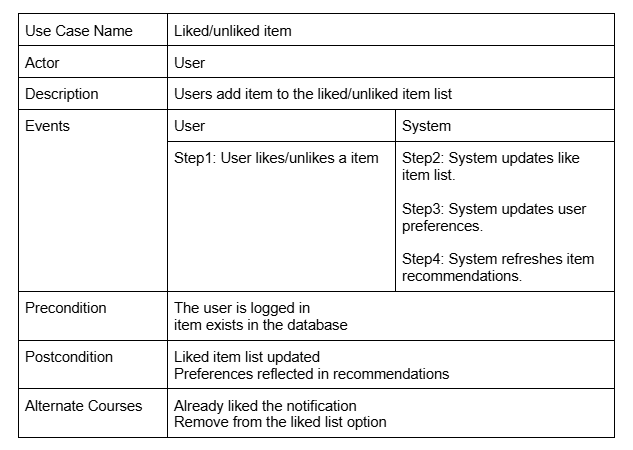
\includegraphics[width=\linewidth]{figures/diagram/Use Case Scenarios/Use Case Scenarios/LikeorUnlike.png}
\end{table}

\begin{table}[H]
    \centering
    \caption{Add Movie to Watch List Sequence Scenario}
    \label{tab:add-movie-watchlist}
    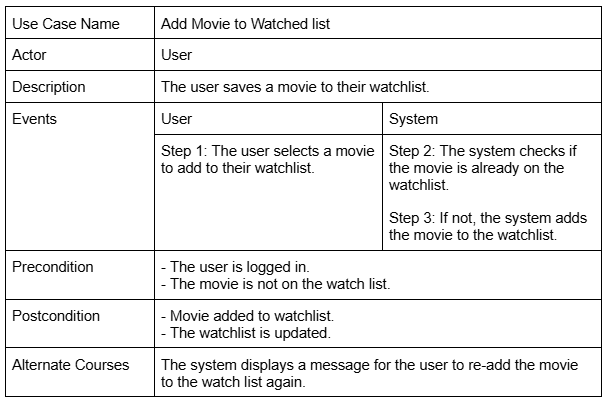
\includegraphics[width=\linewidth]{figures/diagram/Use Case Scenarios/Use Case Scenarios/WatchList.png}
\end{table}

\begin{table}[H]
    \centering
    \caption{Add Game to Wish List Sequence Scenario}
    \label{tab:add-game-wishlist}
    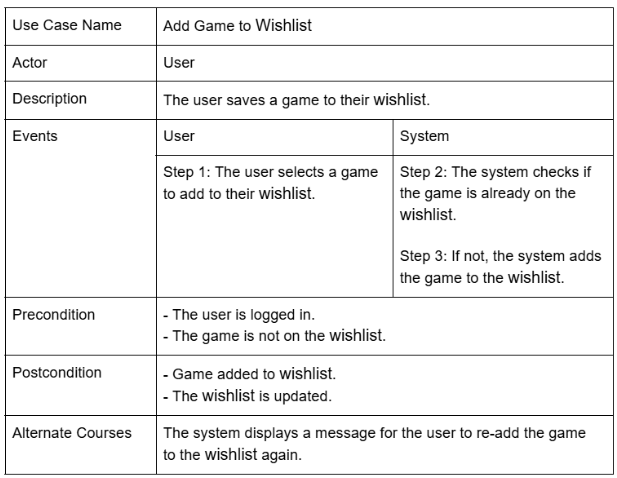
\includegraphics[width=\linewidth]{figures/diagram/Use Case Scenarios/Use Case Scenarios/AddGameToWishList.png}
\end{table}

\begin{table}[H]
    \centering
    \caption{Review Movie Sequence Scenario}
    \label{tab:review-movie}
    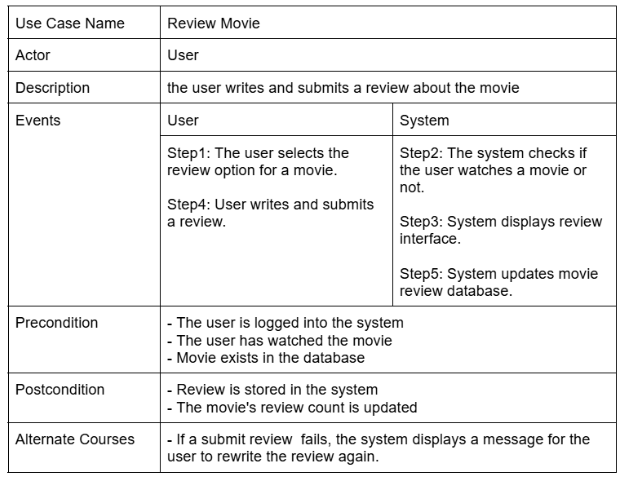
\includegraphics[width=\linewidth]{figures/diagram/Use Case Scenarios/Use Case Scenarios/ReviewMovie.png}
\end{table}

\begin{table}[H]
    \centering
    \caption{Edit Profile Sequence Scenario}
    \label{tab:edit-profile}
    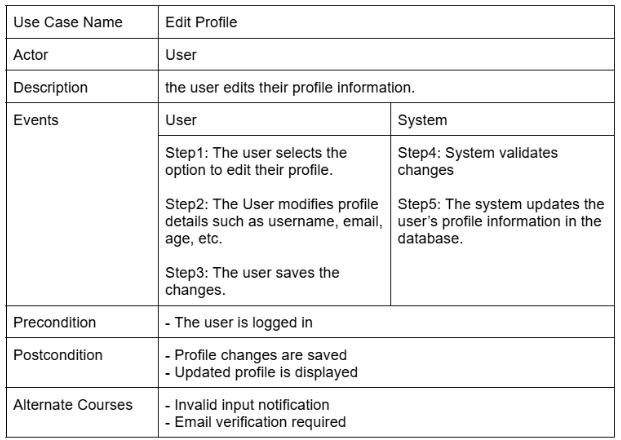
\includegraphics[width=\linewidth]{figures/diagram/Use Case Scenarios/Use Case Scenarios/EditProfile.png}
\end{table}

\begin{table}[H]
    \centering
    \caption{Search Sequence Scenario}
    \label{tab:search}
    
\includegraphics[width=\linewidth]{figures/diagram/Use Case Scenarios/Use Case Scenarios/Search.png}
\end{table}

\begin{table}[H]
    \centering
    \caption{Filter Items Sequence Scenario}
    \label{tab:filter}
    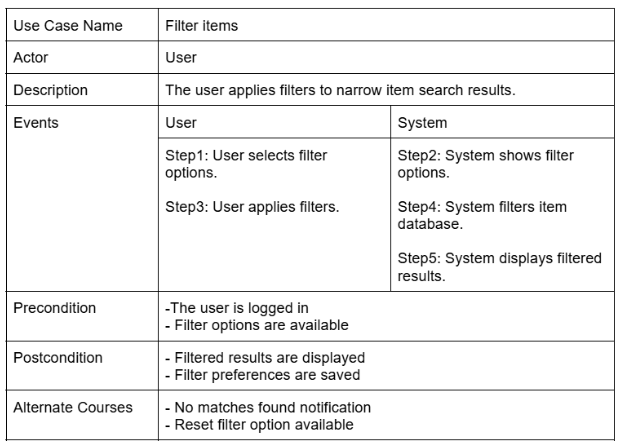
\includegraphics[width=\linewidth]{figures/diagram/Use Case Scenarios/Use Case Scenarios/FilterItems.png}
\end{table}

\begin{table}[H]
    \centering
    \caption{Follow Sequence Scenario}
    \label{tab:follow}
    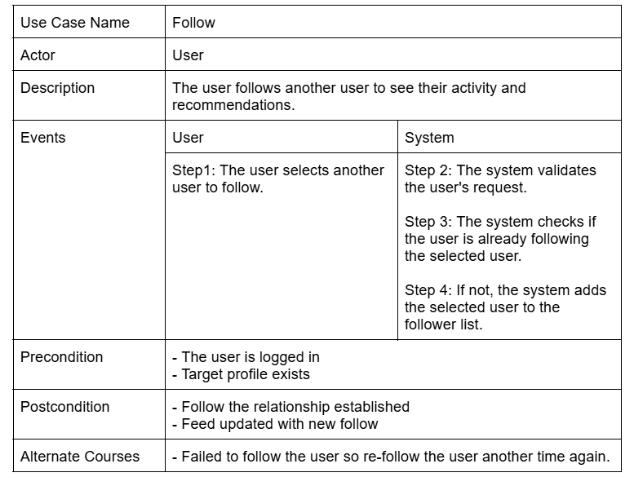
\includegraphics[width=\linewidth]{figures/diagram/Use Case Scenarios/Use Case Scenarios/Follow.png}
\end{table}

\begin{table}[H]
    \centering
    \caption{View Follower Details Sequence Scenario}
    \label{tab:view-followers}
    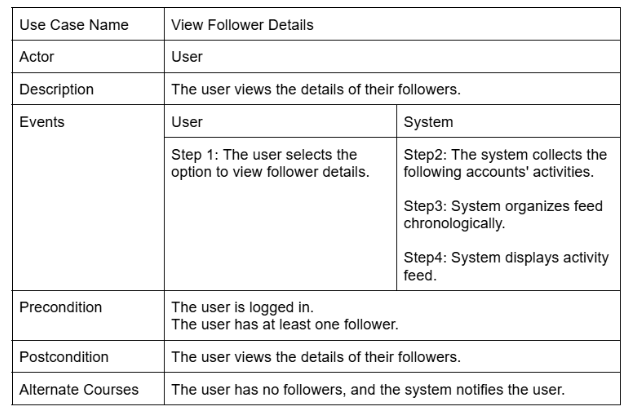
\includegraphics[width=\linewidth]{figures/diagram/Use Case Scenarios/Use Case Scenarios/ViewFollowerDetails.png}
\end{table}

\begin{table}[H]
    \centering
    \caption{Add Items Sequence Scenario}
    \label{tab:add-items}
    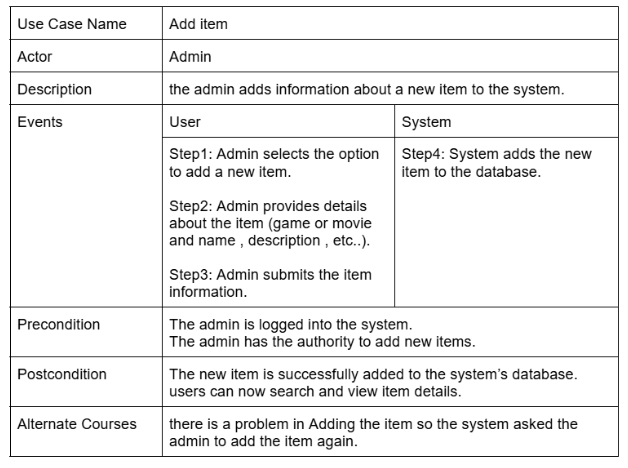
\includegraphics[width=\linewidth]{figures/diagram/Use Case Scenarios/Use Case Scenarios/AddItems.png}
\end{table}

\begin{table}[H]
    \centering
    \caption{View Report Sequence Scenario}
    \label{tab:view-reports}
    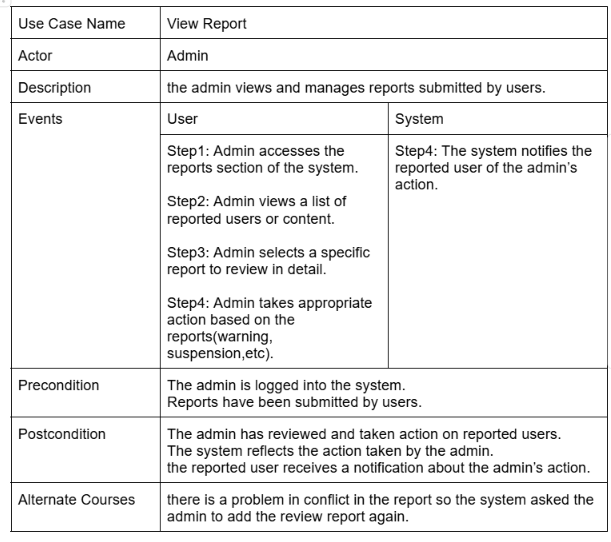
\includegraphics[width=\linewidth]{figures/diagram/Use Case Scenarios/Use Case Scenarios/ViewReports2.png}
\end{table}


\section{Chapter Summary}
\label{sec:system_analysis_summary}
In this chapter, we performed a detailed analysis of the Questro system. We defined the functional and non-functional requirements and utilized standard UML diagrams to visualize the system's structure and behavior. The Context and DFD diagrams established the data boundaries, while the ERD, Class, and Activity diagrams defined the static data and logical flows. Finally, Sequence diagrams illustrated the dynamic logic of key features like the Hybrid Recommendation engine and Sentiment Analysis.